\PassOptionsToPackage{usenames,dvipsnames}{xcolour}
\documentclass[twocolumn,twocolappendix,nofootinbib,iop]{openjournal}

% Add your own macros here:
\pdfoutput=1 %for arXiv submission
\usepackage{amsmath,amssymb,amstext}
\usepackage[T1]{fontenc}
\usepackage{apjfonts}
\usepackage{ae,aecompl}
\usepackage[utf8]{inputenc}
%\usepackage{hyperref}
\usepackage[colorlinks,allcolors=blue]{hyperref}
\usepackage[figure,figure*]{hypcap}
\usepackage{natbib}
\usepackage{url}
\usepackage{mdwlist}
\usepackage{multirow}
\urlstyle{same}
\usepackage{lineno}
\usepackage{fontawesome}



%%%% usepackage{minted}
\usepackage{xcolor}
\definecolor{maroon}{cmyk}{0, 0.87, 0.68, 0.32}
\definecolor{halfgray}{gray}{0.55}
\definecolor{ipython_frame}{RGB}{207, 207, 207}
\definecolor{ipython_bg}{RGB}{247, 247, 247}
\definecolor{ipython_red}{RGB}{186, 33, 33}
\definecolor{ipython_green}{RGB}{0, 128, 0}
\definecolor{ipython_cyan}{RGB}{64, 128, 128}
\definecolor{ipython_purple}{RGB}{170, 34, 255}

\usepackage{listings}


\lstset{
    breaklines=true,
    %
    extendedchars=true,
    literate=
    {á}{{\'a}}1 {é}{{\'e}}1 {í}{{\'i}}1 {ó}{{\'o}}1 {ú}{{\'u}}1
    {Á}{{\'A}}1 {É}{{\'E}}1 {Í}{{\'I}}1 {Ó}{{\'O}}1 {Ú}{{\'U}}1
    {à}{{\`a}}1 {è}{{\`e}}1 {ì}{{\`i}}1 {ò}{{\`o}}1 {ù}{{\`u}}1
    {À}{{\`A}}1 {È}{{\'E}}1 {Ì}{{\`I}}1 {Ò}{{\`O}}1 {Ù}{{\`U}}1
    {ä}{{\"a}}1 {ë}{{\"e}}1 {ï}{{\"i}}1 {ö}{{\"o}}1 {ü}{{\"u}}1
    {Ä}{{\"A}}1 {Ë}{{\"E}}1 {Ï}{{\"I}}1 {Ö}{{\"O}}1 {Ü}{{\"U}}1
    {â}{{\^a}}1 {ê}{{\^e}}1 {î}{{\^i}}1 {ô}{{\^o}}1 {û}{{\^u}}1
    {Â}{{\^A}}1 {Ê}{{\^E}}1 {Î}{{\^I}}1 {Ô}{{\^O}}1 {Û}{{\^U}}1
    {œ}{{\oe}}1 {Œ}{{\OE}}1 {æ}{{\ae}}1 {Æ}{{\AE}}1 {ß}{{\ss}}1
    {ç}{{\c c}}1 {Ç}{{\c C}}1 {ø}{{\o}}1 {å}{{\r a}}1 {Å}{{\r A}}1
    {€}{{\EUR}}1 {£}{{\pounds}}1
}

%%
%% Python definition (c) 1998 Michael Weber
%% Additional definitions (2013) Alexis Dimitriadis
%% modified by me (should not have empty lines)
%%
\lstdefinelanguage{iPython}{
    morekeywords={access,and,break,class,continue,def,del,elif,else,except,exec,finally,for,from,global,if,import,in,is,lambda,not,or,pass,print,raise,return,try,while},%
    %
    % Built-ins
    morekeywords=[2]{abs,all,any,basestring,bin,bool,bytearray,callable,chr,classmethod,cmp,compile,complex,delattr,dict,dir,divmod,enumerate,eval,execfile,file,filter,float,format,frozenset,getattr,globals,hasattr,hash,help,hex,id,input,int,isinstance,issubclass,iter,len,list,locals,long,map,max,memoryview,min,next,object,oct,open,ord,pow,property,range,raw_input,reduce,reload,repr,reversed,round,set,setattr,slice,sorted,staticmethod,str,sum,super,tuple,type,unichr,unicode,vars,xrange,zip,apply,buffer,coerce,intern},%
    %
    sensitive=true,%
    morecomment=[l]\#,%
    morestring=[b]',%
    morestring=[b]",%
    %
    morestring=[s]{'''}{'''},% used for documentation text (mulitiline strings)
    morestring=[s]{"""}{"""},% added by Philipp Matthias Hahn
    %
    morestring=[s]{r'}{'},% `raw' strings
    morestring=[s]{r"}{"},%
    morestring=[s]{r'''}{'''},%
    morestring=[s]{r"""}{"""},%
    morestring=[s]{u'}{'},% unicode strings
    morestring=[s]{u"}{"},%
    morestring=[s]{u'''}{'''},%
    morestring=[s]{u"""}{"""},%
    %
    % {replace}{replacement}{lenght of replace}
    % *{-}{-}{1} will not replace in comments and so on
    literate=
    {á}{{\'a}}1 {é}{{\'e}}1 {í}{{\'i}}1 {ó}{{\'o}}1 {ú}{{\'u}}1
    {Á}{{\'A}}1 {É}{{\'E}}1 {Í}{{\'I}}1 {Ó}{{\'O}}1 {Ú}{{\'U}}1
    {à}{{\`a}}1 {è}{{\`e}}1 {ì}{{\`i}}1 {ò}{{\`o}}1 {ù}{{\`u}}1
    {À}{{\`A}}1 {È}{{\'E}}1 {Ì}{{\`I}}1 {Ò}{{\`O}}1 {Ù}{{\`U}}1
    {ä}{{\"a}}1 {ë}{{\"e}}1 {ï}{{\"i}}1 {ö}{{\"o}}1 {ü}{{\"u}}1
    {Ä}{{\"A}}1 {Ë}{{\"E}}1 {Ï}{{\"I}}1 {Ö}{{\"O}}1 {Ü}{{\"U}}1
    {â}{{\^a}}1 {ê}{{\^e}}1 {î}{{\^i}}1 {ô}{{\^o}}1 {û}{{\^u}}1
    {Â}{{\^A}}1 {Ê}{{\^E}}1 {Î}{{\^I}}1 {Ô}{{\^O}}1 {Û}{{\^U}}1
    {œ}{{\oe}}1 {Œ}{{\OE}}1 {æ}{{\ae}}1 {Æ}{{\AE}}1 {ß}{{\ss}}1
    {ç}{{\c c}}1 {Ç}{{\c C}}1 {ø}{{\o}}1 {å}{{\r a}}1 {Å}{{\r A}}1
    {€}{{\EUR}}1 {£}{{\pounds}}1
    %
    {^}{{{\color{ipython_purple}\^{}}}}1
    {=}{{{\color{ipython_purple}=}}}1
    %
    {+}{{{\color{ipython_purple}+}}}1
    {-}{{{\color{ipython_purple}-}}}1
    {*}{{{\color{ipython_purple}$^\ast$}}}1
    {/}{{{\color{ipython_purple}/}}}1
    %
    {+=}{{{+=}}}1
    {-=}{{{-=}}}1
    {*=}{{{$^\ast$=}}}1
    {/=}{{{/=}}}1,
    literate=
    *{-}{{{\color{ipython_purple}-}}}1
     {?}{{{\color{ipython_purple}?}}}1,
    %
    identifierstyle=\color{black}\ttfamily,
    commentstyle=\color{ipython_cyan}\ttfamily,
    stringstyle=\color{ipython_red}\ttfamily,
    keepspaces=true,
    showspaces=false,
    showstringspaces=false,
    %
    rulecolor=\color{ipython_frame},
    frameround={t}{t}{t}{t},
    numbers=none,
    numberstyle=\tiny\color{halfgray},
    %
    %
    backgroundcolor=\color{ipython_bg},
    %   extendedchars=true,
    %basicstyle=\scriptsize,
    basicstyle=\ttfamily\footnotesize,
    columns=fullflexible,
    keywordstyle=\color{ipython_green}\ttfamily,
}



\newcommand{\nblink}[1]{\href{https://github.com/DifferentiableUniverseInitiative/jax-cosmo-paper/blob/master/notebooks/#1.ipynb}{\faFileCodeO}}
\newcommand{\github}{\href{https://github.com/DifferentiableUniverseInitiative/jax\_cosmo}{\faGithub}}

%%% color Comments 
%% JEC : \FL produces a clash we another definition (but coannot figure out which one)  
\newcommand{\FrL}[1]{{\color{cyan}FL: #1}}
\newcommand{\JZ}[1]{{\color{purple}JZ: #1}}

%%%% new command (JEC)
\newcommand{\nn}{\nonumber}
\newcommand{\numpyro}{\texttt{NumPyro}}
\newcommand{\bydef}{:=}
\newcommand{\jaxcosmo}{\texttt{jax-cosmo}}



\begin{document}
\journalinfo{The Open Journal of Astrophysics}
%\submitted{submitted xxx, revised yyy, accepted zzz}


\title{\jaxcosmo: An End-to-End Differentiable and GPU Accelerated Cosmology Library}

%% use optional labels to link authors explicitly to addresses:
%% \author[label1,label2]{}
%% \address[label1]{}
%% \address[label2]{}

\author{
J.~E. Campagne$^{1,\ast}$, 
F. Lanusse$^2$, 
J. Zuntz$^3$,\\
\jaxcosmo\ contributors}
\thanks{$^\ast$jean-eric.campagne@ijclab.in2p3.fr}

\affiliation{$^1$Université Paris-Saclay, CNRS/IN2P3, IJCLab, 91405 Orsay, France}

%\date{\today}

\begin{abstract}
The recent JAX library has created a new ecosystem from which probabilistic programming software can take enormous benefit: batch acceleration, just-in-time compilation, and automatic optimization of code for different hardware modalities (CPU, GPU, TPU) can provide huge speed-ups to a wide range of different problems. In particular, JAX exposes an \textit{automatic differentiation} mechanism, which can take a python function that uses JAX and return its (vector) derivative.  This gives us the opportunity to apply a range of powerful but otherwise unfeasible algorithms used in Bayesian inference, such as Hamiltonian Monte Carlo (HMC) and Variational Inference. 

To take advantage of these possibilities within cosmology we have developed the \jaxcosmo\ library, which implements background evolution, linear and non linear power spectra (using \texttt{halofit} or the Eisenstein and Hu transfer function), as well as angular power spectra ($C_\ell$) with the Limber approximation for galaxy and weak lensing probes. We discuss algorithms made possible by this library, and present comparisons with the Core Cosmology Library as a benchmark, and run a series of tests using the Dark Energy Survey Year 1 3x2pt analysis with the \numpyro\ library to demonstrate practical usage. 

We show that clear improvements are possible using HMC compared to Metropolis-Hasting, and that the Normalizing Flows using the Neural Transport is a promising methodology.
%{\color{red}
%;in the early phases of Bayesian model development JAZ not sure what this means so I left it out}

\end{abstract}

%\keywords{Suggested keywords}%Use showkeys class option if keyword
                              %display desired
\maketitle


%% \linenumbers

%% main text

\section{Introduction}
Bayesian inference has been widely used in cosmology in the form of Monte Carlo Markov Chains (MCMC) since the work of \citep{2001ApJ...563L..95K,2003MNRAS.341.1084R} and has been the keystone for past and current analysis thanks partly to packages as  \texttt{CosmoMC} \citep{2002PhRvD..66j3511L}, \texttt{CosmoSIS} \citep{2015A&C....12...45Z}, \texttt{MontePython} \citep{2019PDU....24..260B} as well as   \texttt{Cobaya} \citep{2019ascl.soft10019T,2021JCAP...05..057T}; see, for instance, the list of citations to these popular packages for an idea of the wide usage in the community. 

% \footnote{\url{https://cosmologist.info/cosmomc/readme.html}}
% \footnote{\url{http://bitbucket.org/joezuntz/cosmosis}}
% \footnote{\url{https://cobaya.readthedocs.io}}
% \footnote{\url{https://github.com/brinckmann/montepython_public}}

% Note that some direct optimization of likelihood function has also been successfully undertaken for instance for some Planck analysis \citep{2014A&A...566A..54P}, 
Since the development of these MCMC packages, major advances have been made in automatic differentiation (\textit{autodiff}) \citep{2015arXiv150205767G, 2018arXiv181105031M}, a set of technologies for transforming pieces of code into their derivatives.

While these tools have especially been applied to neural network optimization and machine learning in general, they can also enable classical statistical methods that require the derivatives of (e.g. likelihood) functions to operate: we consider such methods in this paper. \textit{Autodiff} has been implemented in widely used libraries like \texttt{Stan} \citep{JSSv076i01}, \texttt{TensorFlow}  \citep{tensorflow2015-whitepaper}, and  \texttt{PyTorch} \citep{NEURIPS2019_9015}. 

A recent entrant to this field is the \texttt{JAX} library\footnote{\url{https://jax.readthedocs.io}} \citep{jax2018github} which has undergone rapid development and can automatically differentiate native \texttt{Python} and \texttt{NumPy} functions, offering a speed up to the development process and indeed code runtimes. \texttt{JAX} offers an easy parallelization mechanism (\texttt{vmap}), and just-in-time compilation (\texttt{jit}) and optimization targetting CPU, GPU and TPU hardware thanks to the \texttt{XLA} library that powers TensorFlow. These attractive features have driven wide adoption of \texttt{JAX} in computational research, and motivate us to consider its usage in cosmology.

\texttt{JAX} contains bespoke reimplementation of packages such as \texttt{jax.numpy} and \texttt{jax.scipy}, as well as example libraries as \texttt{Stax} for simple but flexible neural network development. It has formed the seed for a wider ecosystem of packages, including, for example: 
\texttt{Flax} \citep{flax2020github} a high-performance neural network library, \texttt{JAXopt} \citep{jaxopt_implicit_diff} an hardware accelerated, batchable and differentiable collection of optimizers, \texttt{Optax} \citep{optax2020github} a gradient processing and optimization library, and \numpyro \citep{phan2019composable,bingham2019pyro}, a probabilistic programming language (PPL) that is used in this paper. Other PPL packages such as \texttt{PyMC} \citep{Salvatier2016} have switched to JAX backend in recent versions\footnote{A more exhaustive list and rapidly growing list of packages can be found at \url{https://project-awesome.org/n2cholas/awesome-jax}}.

% I don't think we need all these URLs, it's getting excessive, especially when they have papers:
%\footnote{\url{https://flax.readthedocs.io/}}
% \footnote{\url{https://jaxopt.github.io}}
% \footnote{\url{https://optax.readthedocs.io}}
% \footnote{\url{https://num.pyro.ai}}
% \footnote{\url{https://www.pymc.io/projects/docs/en/stable/installation.html}}
% \footnote{\url{https://www.tensorflow.org/xla}}
% \footnote{\url{https://www.tensorflow.org/}}
% \footnote{\url{https://pytorch.org/docs/}}
% \footnote{\url{https://mc-stan.org/users/documentation}}

In this context we have developed the open source \jaxcosmo\ library\footnote{\url{https://github.com/DifferentiableUniverseInitiative/jax_cosmo}}, which we present in this paper. The package represents a first step in making the powerful features described above useful for cosmology; it implements a selection of theory predictions for key cosmology observables as differentiable JAX functions.


We give an overview of the code's design and contents in Section~\ref{sec-jaxcosmo-design}. We show how to use it for rapid and numerically stable Fisher forecasts in Section~\ref{sec-fisher-forecast}, in more advanced gradient-based cosmological inference with variants of Hamiltonian Monte Carlo and its variant No-U-Turn in Section~\ref{sec:chmc}, and in ML-accelerated Stochastic Variational Inference in Section~\ref{sec-SVI}. We discuss and compare these methods in Section~\ref{sec-discussion} and conclude in Section~\ref{sec-conclusion}.



% \section{JAX: Autograd meets XLA}

\section{Modeling and implementation}
\label{sec-jaxcosmo-design}
In this section, we describe the cosmological modeling provided by \jaxcosmo, and its implementation in JAX. The general design follows that of the Core Cosmology Library (CCL) \citep{2019ApJS..242....2C}, though the present proof-of-concept \jaxcosmo\ does not include as many features and options as CCL.

The cosmological parameters are organised in a JAX \textit{pyTree} container\footnote{\url{https://jax.readthedocs.io/en/latest/jax-101/05.1-pytrees.html}} \texttt{jc.Cosmology} where \texttt{jc} hereafter stands for \jaxcosmo. This container allows one to use \textit{autodiff} and \texttt{vmap} transparently. The present set of exposed parameters is: $\Omega_{cdm}$ the cold dark matter density fraction, $\Omega_b$ the Baryonic matter density fraction, $h$ the Hubble constant divided by $100$~km/s/Mpc, $n_s$ the primordial scalar perturbation spectral index, $\sigma_8$ the variance of matter density perturbations at an $8$~Mpc/h scale, $\Omega_k$ the curvature density fraction, $w_0$ the first order term of dark energy equation and $w_a$ the second order term of dark energy equation of state. Notably, \texttt{jc.Planck15} instantiates a set of cosmological parameters inspired from the Planck 2015 results \citep{2016A&A...594A..13P}. 

\subsection{Background cosmology}

The computation of the evolution of the cosmological background follows a typical implementation of a Friedmann equation (\citealp[see e.g.][]{2005A&A...443..819P}):
\begin{equation}
    E^2(a) = \frac{\mathrm{H}^2(a)}{\mathrm{H}^2_0} = \Omega_m a^{-3} + \Omega_k a^{-2} + \Omega_{de} e^{f(a)}
\end{equation}
with $a=1/(1+z)$ the scale factor related to the redshift $z$, $H(a)=\dot{a}/a$ the Hubble parameter with $\mathrm{H}_0$ its present day value, $\Omega_m= \Omega_{cdm}+\Omega_b$, $\Omega_{de}=1-\Omega_k-\Omega_m$, and 
\begin{equation}
    f(a) = -3 (1 + w_0 + w_a) \ln(a) + 3 w_a (a - 1)
\end{equation}
Notably, the relativistic contributions of massless neutrinos and photon radiation, as well as the massive neutrino contribution are presently neglected. From these expressions, in \texttt{jc.background}, are computed the different cosmological distance functions. Notably, the radial comoving distance
\begin{equation}
     \chi(a) =  R_H \int_a^1 \frac{da^\prime}{{a^\prime}^2 E(a^\prime)}
     \label{eq:radial_comoving}
\end{equation}
with $R_H$ the Hubble radius. Using the scale factor ($a$) redshift ($z$) relationship, $\chi$ can be viewed as a function of $z$. 
%
\subsection{Growth of perturbations}
%
Currently, \jaxcosmo\  implements the \citet{Eisenstein_1998} transfer function and non-linear features through the \textit{halofit} model by \cite{2012ApJ...761..152T} or \cite{2003MNRAS.341.1311S} without the neutrino contribution introduced by \cite{10.1111/j.1365-2966.2011.20222.x}. No Baryon feedback modeling is considered yet. To perform \textit{autodiff} we have implemented various tools as differentiable ODEs using the Runge-Kutta algorithm, as well as Simpson quadrature and the Romberg algorithm for numerical integration.

%Future version of the library would offer the possibility to call a JAX emulator of the Cosmic Linear Anisotropy Solving System \citep{2011JCAP...07..034B}. \JZ{How close is this to being usable? If it's just an idea or an early prototype then skip this paragraph.}
%
\subsection{Angular power spectra}
%
\jaxcosmo\ is currently focused on predicting projected 2D Fourier-space 2pt galaxy lensing, clustering, and cross correlations, the $C_\ell$ angular power spectra that are a primary target of upcoming photometric surveys. The details of the implementation is in \texttt{jc.angular\_cl} which deals with the mean and Gaussian covariance matrix computations.

To make a bridge to these observables, two \textit{pyTree} objects are implemented: \texttt{NumberCounts} and \texttt{WeakLensing} tracers for galaxy clustering and weak lensing samples, with each instance of each representing a single tomographic redshift bin's number density. These tracers are implemented as two kernel functions:

\begin{description}
\item[\texttt{NumberCounts}]
    \begin{equation}
        K_i(z) = n_i(z)\ b(z)\ H(z)
    \end{equation}
where $n_i(s)$ is the redshift distribution of the sample (eg. \texttt{jc.redshift.kde\_nz} function), $b(z)$ a galaxy bias function (see  \texttt{jc.bias.constant\_linear\_bias}). No redshift space distortions are taken into account.

\item [\texttt{WeakLensing}]
    \begin{multline}
 K_i(z) = \left( \frac{3 H_0^2\Omega_m}{2 c} \right) \left(\frac{(\ell+2)!}{(\ell-2)!} \right)^{1/2}\times 
 \\  (1+z)\ \chi(z) \int_z^\infty p_i(z^\prime)\ \frac{\chi(z^\prime)-\chi(z)}{\chi(z^\prime)}\ dz^\prime + K_{IA}(z)
    \end{multline}
where $K_{IA}(z)$ is an optional kernel function to deal with the Intrinsic Alignment. The implementation of this term currently follows \citet{2011A&A...527A..26J}, and is given by:
\begin{equation}
    K_{IA}(z) =   \left(\frac{(\ell+2)!}{(\ell-2)!}\right)^{1/2}\ p_i(z)\ b(z)\  H(z)\ \frac{C\  \Omega_m}{D(z)}
\end{equation}
with $C\approx 0.0134$ a dimensionless constant and $D(z)$ the growth factor of linear perturbations.
\end{description}

Notice that all described kernel functions can be also viewed as function of the scale factor $a$ or as function of the radial comoving distance $\chi$. 

From these tracer objects, the angular power spectra $C_\ell^{ij}$ for the probes $(i,j)$ and for redshift bin window selections are computed in the first order Limber approximation \citep{PhysRevD.78.123506}:
%\JZ{Discuss the implementation of the Limber integral here. Maybe move down the bit in the growth of perturbations section?}
\begin{align}
    C_\ell^{i,j} \approx \left(\ell+\frac{1}{2}\right)^{m_i+m_j}\int\frac{d\chi}{c^2\chi^2}K_i(\chi)K_j(\chi)\,P\left(k=\frac{\ell+1/2}{\chi},z\right),\label{eq:Cell_limber}
\end{align}
with $P(k,z)$ the power spectra computed using the growth of perturbation models described above and a primordial power spectra scaling according to
\begin{equation}
    P(k) = A k^{n_s}
\end{equation}
The normalisation $A$ is computed using the $\sigma_8$ parameter as 
\begin{equation}
    A = \sigma_8^2 \times \left(\frac{1}{2 \pi^2} \int_0^\infty \frac{dk}{k} k^3 P(k,z) W^2(kR_8) \right)^{-1}
\end{equation}
with $R_8 = 8$ in unit of Mpc and $W(x)$ is related to the $j_1$ spherical Bessel function as
\begin{equation}
    W(x) = \frac{3j_1(x)}{x}
\end{equation}
Finally, the factors $m_i$ are equal to $(0,-2)$ for the \texttt{NumberCounts}, \texttt{WeakLensing} related kernels, respectively.

Remarkably, all the integrals involved in these computations can be  differentiated with respect to the cosmological parameters thanks to \textit{autodiff} and the implementation of the above mentioned integration quadrature.  An example is given in the context of DES Y1 3x2pts analysis (Appendix~\ref{app-DESY1}).
%
\subsection{Validation against the Core Cosmology Library (CCL)}
%
To illustrate the different features available with the present version of the library (\jaxcosmo\ \texttt{0.1rc9}, which is available in the Python Package Index PyPI\footnote{\url{https://pypi.org/}}), we have written a  companion notebook \nblink{CCL_comparison} to make a comparison with the well-established  Core Cosmology Library \citep{2019ApJS..242....2C}\footnote{\url{https://ccl.readthedocs.io}, version \texttt{2.5.1}.}. As examples, the Figures \ref{fig:chi_comparison},
\ref{fig:halofit_comparison} and \ref{fig:Cell_comparison}
show the radial comoving distance (Eq.~\ref{eq:radial_comoving}), the non linear matter power spectrum computation using the \texttt{halofit} fitting function and the angular power spectrum for galaxy-galaxy lensing (Eq.~\ref{eq:Cell_limber}) using the \texttt{NumberCounts} and \texttt{WeakLensing} kernel functions. The relative differences between the two libraries are at the level of few $10^{-3}$ or better.

These numerical differences are mostly due to different choices of integration methods and accuracy parameters (eg. quadrature number of points). Increasing these parameters lead to performance degradation for \jaxcosmo\ as it increases the XLA compilation memory requirements significantly, especially for the angular power spectra computation. Since these differences are likely to be within the tolerance of the current generation of cosmological surveys, this trade-off is an acceptable one.
 

\begin{figure}
    \centering
    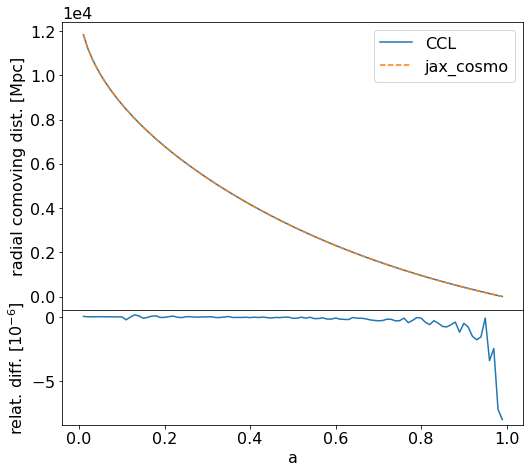
\includegraphics[width=\columnwidth]{figures/comp_radial_com_dist.png}
    \caption{Comparison of the radial comoving distance between CCL and \jaxcosmo. More plots are available in the  companion notebook \nblink{CCL_comparison}.} 
    \label{fig:chi_comparison}
\end{figure}
\begin{figure}
    \centering
    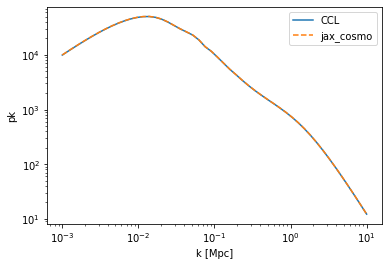
\includegraphics[width=\columnwidth]{figures/halofit_pk.png}
    \caption{Comparison of the non-linear matter power spectrum (\textit{halofit} function) between CCL and \jaxcosmo. Is also shown the linear power spectrum.}     \label{fig:halofit_comparison}
\end{figure}
\begin{figure}
    \centering
    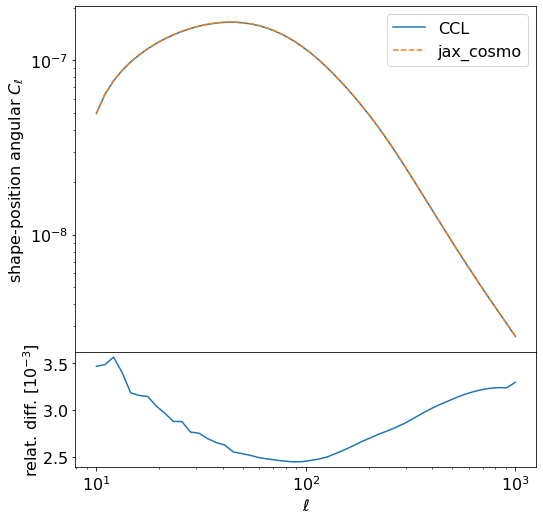
\includegraphics[width=\columnwidth]{figures/comp_Cell_shape_pos.png}
    \caption{Comparison of the shape-position angular power spectrum between CCL and \jaxcosmo.} 
    \label{fig:Cell_comparison}
\end{figure}


\section{Application: Fisher Forecasting}
\label{sec-fisher-forecast}
% illustrates why autodiff is interesting from several points of view

\FrL{Add description of problem and small demos}


%JEC 5 August 22: not sure that should be given here as we have an Appendix for that and the main application described in the following sections concern DES Y1. 
%\subsection{DES Y1 setting}
% Here we describe the data and 3x2pt model for DES Y1 
% In this section, we adopt as a setting a DES Y1 3x2pt-like analysis. 


\subsection{Instantaneous Fisher Forecasts}
In this section, we illustrate with a purely fictional case study, the computation of the Fisher matrix \citep{1997ApJ...480...22T,Stuart1991} by two methods thanks to the \textit{autodiff} ability of JAX. For the detailed implementation, the reader is invited to have a look at the following companion notebook \nblink{Simple-Fisher}. In this use-case we use four tracers redshift distributions: two to define \texttt{WeakLensing} kernels and two for \texttt{NumberCounts} kernels. Then, the $10$ angular power spectra $C_\ell^{p,q}$ ($p,q:1,\dots,4$) are computed for $50$  logarithmically spaced angular moments between $10$ and $1000$ using Equation \ref{eq:Cell_limber}. The Gaussian covariance matrix is computed simultaneously. A dataset is obtained from the computation of the $C_\ell^{p,q}$ with a fiducial cosmology. Then, the following snippet shows the log likelihood function $\mathcal{L}(\theta)$ implementation considering a constant covariance matrix ($\theta$ stands for the set of cosmological parameters). 
%\begin{minted}[fontsize=\footnotesize]{python}
\begin{lstlisting}[language=iPython]
@jax.jit
def likelihood(p):
    # Create a new cosmology at these parameters
    cosmo = jc.Planck15(Omega_c=p[0], sigma8=p[1])
    # Compute mean and covariance of angular Cls
    mu, C = jc.angular_cl.gaussian_cl_covariance_and_mean(cosmo, ell, tracers, sparse=True)
    # Return likelihood value assuming constant covariance, so we stop the gradient
    # at the level of the precision matrix, and we will not include the logdet term
    # in the likelihood
    P = jc.sparse.inv(jax.lax.stop_gradient(C))
    r = data - mu
    return -0.5 * r.T @ jc.sparse.sparse_dot_vec(P, r)
\end{lstlisting}
%\end{minted}
The \texttt{jc.sparse} functions are implementation of block matrix computations: sparse matrix is represented as a 3D array of shape $(n_y, n_x, n_{diag})$ composed of $n_y \times n_x$ square blocks of size $n_{diag} \times n_{diag}$.  The \texttt{jax.jit} decorator is there to build a compiled version of the function at the first use. The goal is to obtain the 1-sigma contour forecast of the two parameters ($\Omega_c, \sigma_8$). To do so, we use the Fisher matrix computation. One way is to use the Hessian of the log-likelihood as follows
\begin{equation}
F_{i,j} = - \frac{\partial^2\mathcal{L}(\theta)}{\partial \theta_i \partial \theta_j}
\qquad (\theta_1=\Omega_c, \theta_2=\sigma_8)
\label{eq:fisher_way1}
\end{equation}
which is mostly  1-line JAX code
\begin{lstlisting}[language=iPython]
hessian_loglik = jax.jit(jax.hessian(likelihood))
F = - hessian_loglik(params)
\end{lstlisting}
An other way uses the computation of the Fisher matrix when the likelihood is a Gaussian distribution as ii is the case above. First, we define a function that computes the mean  $\mu(\ell; \theta)$, and it follows that the Fisher matrix element reads
\begin{equation}
    F_{i,j} = \sum_\ell \frac{\partial \mu(\ell)}{\partial \theta_i}^T C^{-1}(\ell)\frac{\partial \mu(\ell)}{\partial \theta_j}
    \label{eq:fisher_way2}
\end{equation}
where $C^{-1}(\ell)$ is the covariance matrix computed with the fiducial cosmology. In this case one needs also just 1-line of JAX code 
\begin{lstlisting}[language=iPython]
F = jc.sparse.dot(dmu.T, jc.sparse.inv(cov), dmu)
\end{lstlisting}

The two methods agree perfectly as shown on Figure \ref{fig:simple_fisher_1}.
\begin{figure}
    \centering
    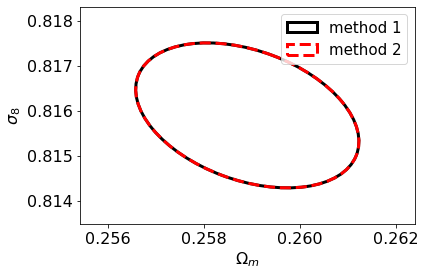
\includegraphics[width=0.7\columnwidth]{figures/simple_fisher_1.png}
    \caption{Comparison of the two methods to compute the Fisher matrix (Eqs.\ref{eq:fisher_way1},\ref{eq:fisher_way2}).} 
    \label{fig:simple_fisher_1}
\end{figure}
%
It is worth to notice that in the two above methods of Fisher matrix computations, the user does not need to take care of particular parameter to compute the 1st or 2nd order derivatives. This is in contrast to the cases where one deals with finite difference methods. AS an illustration, we have used the CCL library to compute the Fisher matrix via Equation \ref{eq:fisher_way2}. To do so, the Jacobian ($\partial \mu/\partial\theta_\alpha$) is computed with centered  order 4 finite differences available in the \texttt{Numdifftools} Python package\footnote{\url{https://numdifftools.readthedocs.io}}. Using the spacing parameter values ($10^{-6}$, $10^{-2}$, $10^{-1}$) one obtains three different approximation of the 1-sigma contours as shown on Figure \ref{fig:simple_fisher_2}. One notices that the contour that agrees quite well with the \jaxcosmo\ one, is obtained with the spacing parameter equals to $10^{-2}$ which implies that the user has to  tune this parameter carefully. Although very simple, this case study exhibits the intrinsic limitation of finite difference methods for computing the Fisher matrix as it as been shown for instance in a more advanced case study in reference \citet{2021arXiv210100298B}.
\begin{figure}
    \centering
    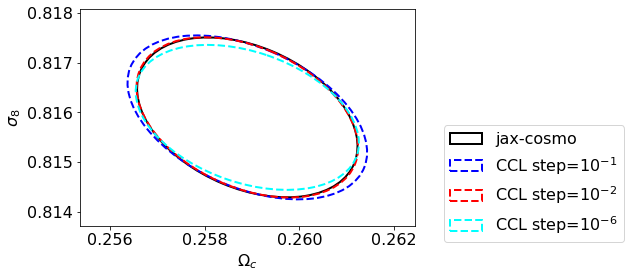
\includegraphics[width=\columnwidth]{figures/simple_fisher_2.png}
    \caption{Computations of the Fisher matrix (Eq.\ref{eq:fisher_way1}) using the CCL library for the angular power spectra estimation and finite difference method to get the Jacobian  with different spacing parameters ($10^{-6}$, $10^{-2}$, $10^{-1}$). For comparison, the contour obtained with \jaxcosmo\ is reproduced from Figure \ref{fig:simple_fisher_1} in black.} 
    \label{fig:simple_fisher_2}
\end{figure}
%
\subsection{Survey Optimization by FoM Maximization}
\label{sec-FOM-optimisation}
% Needs to mention the tomo challenge, mention that we can backpropagate through a NN and the cosmology model
% Maybe this can be only mentioned in the discussion.

Fisher forecasts are also commonly used in survey and analysis strategy strategy, where running a full posterior analysis for each possible choice would be unfeasible. The inverse area of a projection of a Fisher matrix in parameters of interest can be used as a metric for survey constraining power, such as in the Dark Energy Task Force report \citep{2006astro.ph..9591A}.

\jaxcosmo\ was used in a recent example of such a process, for the  the LSST-DESC 3x2pt tomography optimization challenge \citep{2021OJAp....4E..13Z}, where the best methodology for assignment of galaxies to tomographic bins was assessed using several such figures of merit and related calculations. The \jaxcosmo\ metric proved to be stable and fast.



\subsection{Massive Optimal Compression in 3 Lines}

\FrL{Here we can implement MOPED for the compression}

Once the Fisher matrix can be safely estimated, one can use the MOPED\footnote{Massively Optimised Parameter Estimation and Data compres-
sion} algorithm \citep{2000MNRAS.317..965H,2016PhRvD..93h3525Z, 2017MNRAS.472.4244H}. In the case of the constant covariance matrix the algorithm leads to a  lossless compression which reduces possibly large data vector $x$ of size $N$ to $M$ numbers, where $M$ is the number of parameters $\theta_i$ considered. For instance, in the previous section, $N=500$ as $x=(C_\ell^{p,q})$ and $M=2$ for $(\Omega_c,\sigma_8)$. The algorithm computes by iteration $M$ vectors of size $N$ such that (taking the notation of the previous section)
\begin{equation}
    b_i = \frac{C^{-1}\mu_{,i}-\sum_{j=1}^{i-1}(\mu_{,j}^T b_j)b_j}{\sqrt{F_{i,i}-\sum_{j=1}^{i-1}(\mu_{,j}^T b_j)^2}}
\end{equation}
where $\mu_{,i}=\partial \mu/\partial \theta_i$ ($i=1,\dots,M$). The vectors $(b_i)_{i\leq M}$ satisfy the following orthogonality constraint
\begin{equation}
    b_i^T C b_j = \delta_{i,j}
\end{equation}
The algorithm is similar to the Gram-Schmidt process with a constant covariance matrix $C$to define the scalar product $\langle b_i, b_j\rangle$. Then, the original data set $x=(C_\ell^{p,q})_{p,q,\ell}$ is compressed in a data set composed of $M$ numbers $(y_i)_{i\leq M}$ according to
\begin{equation}
    y_i = b_i^T x
\end{equation}
These numbers are uncorrelated and of unit variance and $(y_i)_{i\leq M}$ is a set of sufficient statistic for the set of parameters $(\theta_i)_{i\leq M}$, $y_i$ contains the maximum information about the parameter $\theta_i$.The case where the covariant matrix depends upon the parameters is discussed by  \citet{2017MNRAS.472.4244H}.

The net gain of MOPED algorithm is to eliminate the need of large covariance matrix inversion of size $N\times N$ requiring $O(N^3)$ operations. This inversion takes place not only for the Fisher matrix computation (Eq.~\ref{eq:fisher_way2}, but more importantly in the log-likelihood computation (see the snippet of the previous section). The MOPED algorithm reduces the complexity to $O(M)$ operations. 

To give an illustration here is a snippet that use the mock data set and the results of the Fisher matrix computation as in the previous section, to get the MOPED compressed data set composed of two numbers $(y_0,y_1)$ with maximal information on $(Omega_c, \sigma_8)$ respectively:  
\begin{lstlisting}[language=iPython]
# Orthogonal vectors
b0 = jc.sparse.dot(C_inv,dmu[:,0])/jax.numpy.sqrt(F[0,0])
a = dmu[:,1].T @ b0
b1 = (jc.sparse.dot(C_inv,dmu[:,1]) - a * b0)/jax.numpy.sqrt(F[1,1]-a*a)
# MOPED vector
y0 = b0.T @ data
y1 = b1.T @ data
\end{lstlisting}
Then, the log-likelihood can easily be implemented as followed
\begin{lstlisting}[language=iPython]
@jax.jit
def compress_likelihood(p):
    # Create a new cosmology at these parameters
    cosmo = jc.Planck15(Omega_c=p[0], sigma8=p[1])
    # Compute mean Cl
    mu = jc.angular_cl.angular_cl(cosmo, ell, tracers).flatten()
    # likelihood using the MOPED vector
    return -0.5 * ((y0 - b0.T @ mu)**2 + (y1 - b1.T @ mu)**2)
\end{lstlisting}
%
\section{Application: Classical Hamiltonian Monte Carlo}
\label{sec:chmc}
%
In the following sections we review some statistical methods used to make the cosmological parameter inference with \jaxcosmo. We have used a variant of Hamiltonian Monte Carlo knows as \textit{No-U-Turn} (NUTS) and NUTS after a \textit{Neural Transport} perform using a \textit{Stochastic Variational Inference} (aka SVI). All  the methods have been implemented using the \numpyro\ probabilistic programming language (PPL). 
%
%
%
\subsection{Vanilla HMC}
%
% Show Joe's vanilla HMC results against Cobaya
Hamiltonian Monte Carlo (HMC) is an MCMC-type method particularly suited to drawing
samples from high dimensional parameter spaces.  It was introduced in \citep{1987PhLB..195..216D}
and developed extensively since.  See \citet{betancourt} for a full review; we describe
very basic features here.

HMC samples spaces by generating particle trajectories through the space, using the log-posterior as the negative potential energy of a particle at each point $q$ in the space. Associated to $q$, we introduce an auxiliary $p$ variable in the spirit of Hamiltonian momentum such that
\begin{equation}
- \log{\cal P}(q) = V(q) + cte; \quad H(q,p) = V(q) + U(p)
\end{equation}
where $U(p)$ is a sort of \textit{kinetic} term defined by 
\begin{equation}
U(p) = p^T M^{-1} p
\end{equation}
At each sample, a trajectory is initialized with a random momentum $p$, and then integrated using Hamilton's equations with a numerical integration (so called \textit{leapfrog} algorithm):
\begin{align}
\frac{\mathrm{d}p}{\mathrm{d}t} &= - \frac{\partial V}{\mathrm{d} q} = \frac{\partial \log{\cal P}}{\mathrm{d} q}\\
\frac{\mathrm{d}q}{\mathrm{d}t} &= + \frac{\partial U}{\mathrm{d} p} = M^{-1} p
\end{align}
where $M$ is a mass matrix which should be set to approximate the covariance of the posterior. This is also used to set the scale of the random initial velocities.

Formally, the set of $n_\mathrm{dim}$ moment are treated as new parameters, and after 
some number of integration steps a final point in the trajectory is compared to the initial one,
and a Metropolis-Hastings acceptance criterion on the total energy $H(q,p)$ is applied. If the trajectory is perfectly simulation then this acceptance is unity, since energy is conserved; applying it allows
a relaxation to the integration accuracy.

That gradients $\partial \log{\cal P} / \mathrm{d} q$ can be estimated using finite differencing,
but this typically requires at least $4 n_{\mathrm{dim}} + 1$ posterior evaluations per point, greatly slowing it
in high dimension, and as with the Fisher forecasting is highly prone to numerical error. Automatically
calculating a Hessian, as in \jaxcosmo, makes it feasible and efficient.

The tricky point is that the \textit{leapfrog} algorithm needs tuning to set the number of steps as well as the step size of integration. The next section addresses this problem thanks to the No-U-Turn HMC version.

%Below we show an example set of HMC constraints using \jaxcosmo\ to constrain a simulated
%Dark Energy Survey Year One (DES-Y1) lensing and clustering-like (3x2pt) likelihood, using 21 parameters\footnote{We omit the 
%five clustering sample photometric redshift parameters}.  We re-parametrize the space to unit mass using the Cholesky 
%decomposition
%of the covariance as estimated with an initial Fisher matrix; this lets us reflect the trajectories when they reach the
%edge of the parameter space, as recommended in \citep{NIPS2015_8303a79b}.  We use a fixed number (25) of integration steps and 
%a fixed integration period (0.02), this was chosen heuristically to give a reasonable acceptance rate, but is likely to be
%far from optimal.  We compare to the highly-optimized \texttt{Cobaya} 
%Metropolis-Hastings implementation  %\citep{cobaya2,cobaya1} JEC it may preferable to have a single up to date reference in JCAP
%\citep{2019ascl.soft10019T,2021JCAP...05..057T}, initializing it with the Fisher matrix as a proposal and
%tuning thereafter.  We ran two processes for each sampler, with four CPU threads per process.
%
%The Hamiltonian sampler required around half the number of samples as the Metropolis (70,000 vs 140,000) to reach approximately the same
%convergence, as tested by the Gelman-Rubin test \citep{gelman}, though each sample was itself a few times slower
%on a CPU.  This proof-of-principle example can certainly be hugely improved using various extensions to HMC such as No U-Turn Sampling \citep{nuts} or sampling from the entire trajectories \cite{betancourt}.  On next generation GPU high-performance systems, the advantage will be large.
%
%\begin{figure}
%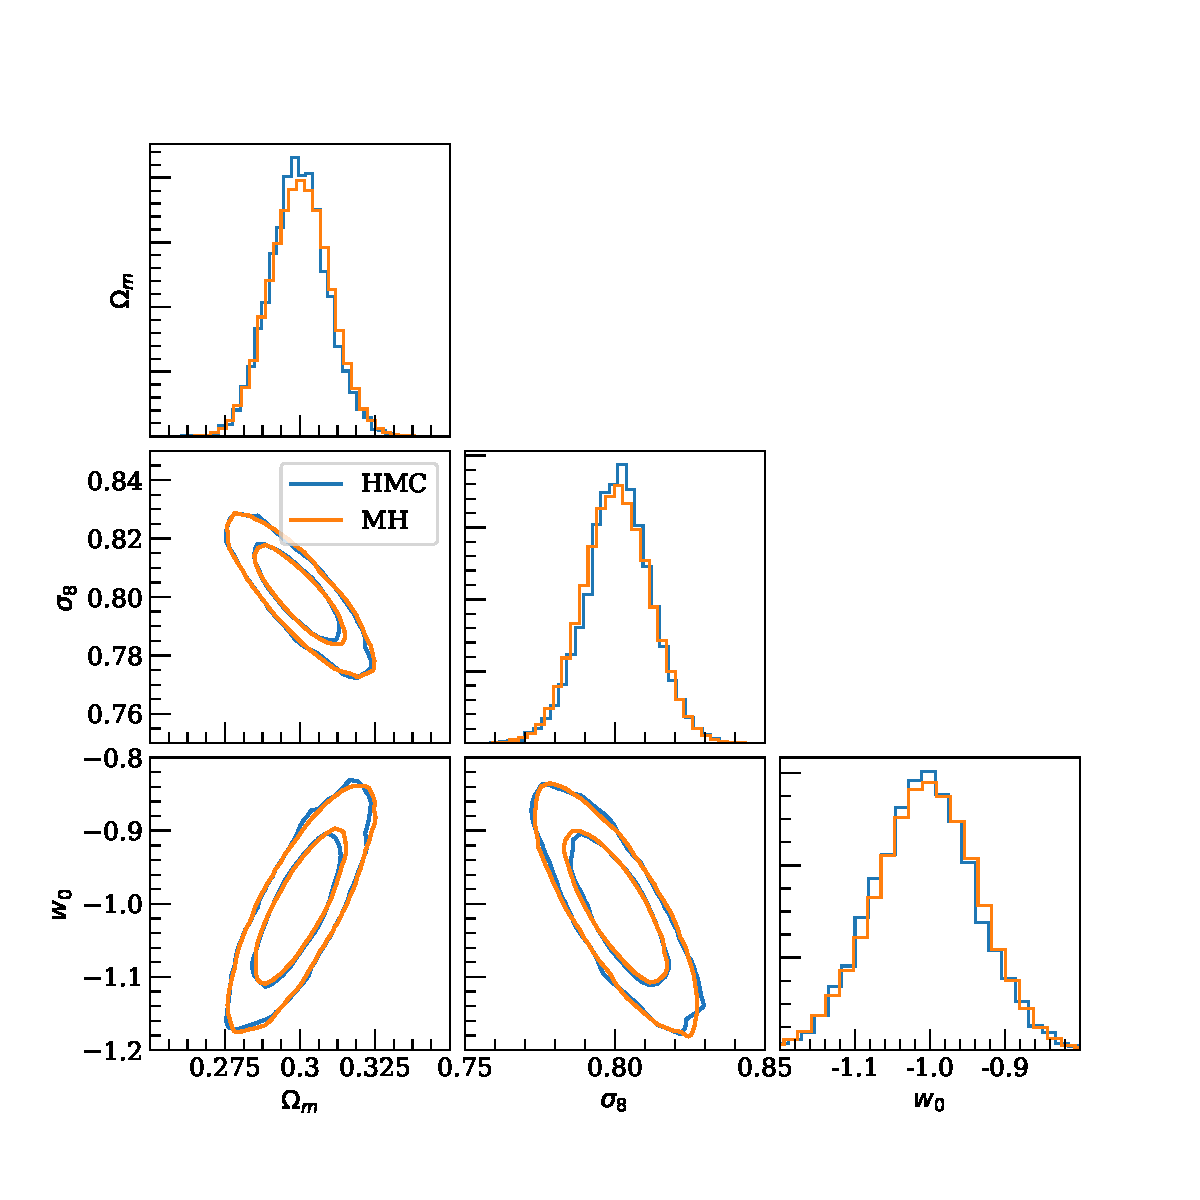
\includegraphics[width=0.95\columnwidth]{figures/hmc.pdf}
%\caption{Constraints on three of the 21 parameters of a simulated DES-Y1 3x2pt likelihood, using a simple Hamiltonian
%Monte Carlo sampler with \jaxcosmo\ (blue), compared to the \texttt{Cobaya} Metropolis-Hastings sampler (orange).}
%\end{figure}
%
%
%We note that a full Boltzmann code accurate enough to calculate the CMB spectra to Planck \citep{planck18}
%or future \citep{s4,simons} accuracy is currently beyond the scope of this project.  
%If this is needed then HMC could use a fast approximation to a CMB theory spectrum, and importance sampling applied to the complete chain.

\subsection{NUTS}
\label{sec-NUTS}
%
% Show the advantage of using NUTS 
% look at difference in efficiency in terms of how many times we need to call the model.

The No-U-Turn (aka NUTS))  variant of the traditional HMC sampler has been introduced in reference \citep{nuts}. It aims to help finding a new point  $x_{i+1}$ from  the current $x_i$. Namely, the root algorithm of HMC deals with the \textit{leapfrog} integration which requires to set two main parameters: $\varepsilon$ the step size and $L$ the number of steps. As stated by the authors, NUTS  uses a recursive algorithm to build a set of likely candidate samples that spans a wide swath of the target distribution, stopping automatically when it starts to double back and retrace its steps. So, in a automatic manner the parameter $L$ is adjusted to produce statistically  a new point $x_{i+1}$ independent from $x_i$, at the expense of the increase the number of model calls. The user has to set a new  parameter  (\texttt{max\_tree\_depth}) which gives in power of $2$ the maximal number of model calls at each generation.

Both sampler HMC and NUTS are available in the \numpyro\ library: \texttt{NUTS} is inherited from \texttt{HMC} which in turns is inherited from the generic \texttt{MCMC} class.  After the forward model creation for the DES-Y1 3x2pts exercise described in Appendix~\ref{app-DESY1}, we have performed 
\begin{itemize}
    \item first a reparametrisation of the latent variable uniform priors (Table~\ref{tab-DESY1}) to use a unified uniform prior $\mathcal{U}[-5,5]$;
    \item second for the warm-up phase we ask for mass matrix optimisation with essentially a diagonal form but with a block structure for the following sets of parameters $(\Omega_b,\Omega_c,\sigma_8,w_0,h)$ and $(b_i)_{i:1\dots5}$. This matrix structuring is motivated by the expected degree of correlation of the concerned parameters as can be shown for instance in Figure \ref{fig_cobaya_NUTS_SVI_bis}.
\end{itemize}
The NUTS sampler have been running with 16 chains of 1,000 samples each (\texttt{vectorized} option) after a warm-up phase consisting of 200 samples, and the \texttt{max\_tree\_depth} has been set to 7 by default (ie. 128 steps for each iteration). The experiments have been undertaken on a single GPU either a NVidia Titan Xp (12GB RAM) on a desktop or a NVidia V100 (32GB RAM) at the IN2P3 Computing Centre\footnote{\url{https://cc.in2p3.fr/en/}}. The elapse time for these experiments was 20 hours.

The results in terms of relative effective sample sizes (aka "ESS") are detailed in Table~\ref{tab-ESS-NUTS_SVI-1} while the confidential level (CL) contours are presented in Figure \ref{fig_cobaya_NUTS_SVI}. One notices the dramatic improvement of the ESS by about a factor 10 using the NUTS sampler compared to the highly-optimized \texttt{Cobaya}  Metropolis-Hastings implementation \citep{2019ascl.soft10019T,2021JCAP...05..057T} which has last about 40 hours on CPU to generate 70,000 samples. The CL contours are also in very good agreement. It is worth to point out that the mass matrix structuring operation is a very effective as it increases the sampling efficiency by about a factor 2.   Anticipating the Section~\ref{sec-Neural-Reparametrisation} devoted to the Neural Transport which is an effective solution to validate the model with fewer samples, we have used a NUTS sampling with \texttt{max\_tree\_depth=5} those elapse time is 5 hours. This clearly shows a linear scaling with respect to the number of steps per iteration keeping the sampling efficiencies at a high level (see Table~\ref{tab-ESS-NUTS_SVI-1}), then the user is highly encouraged to tune this critical parameter. 
%
\begin{figure*}
\centering
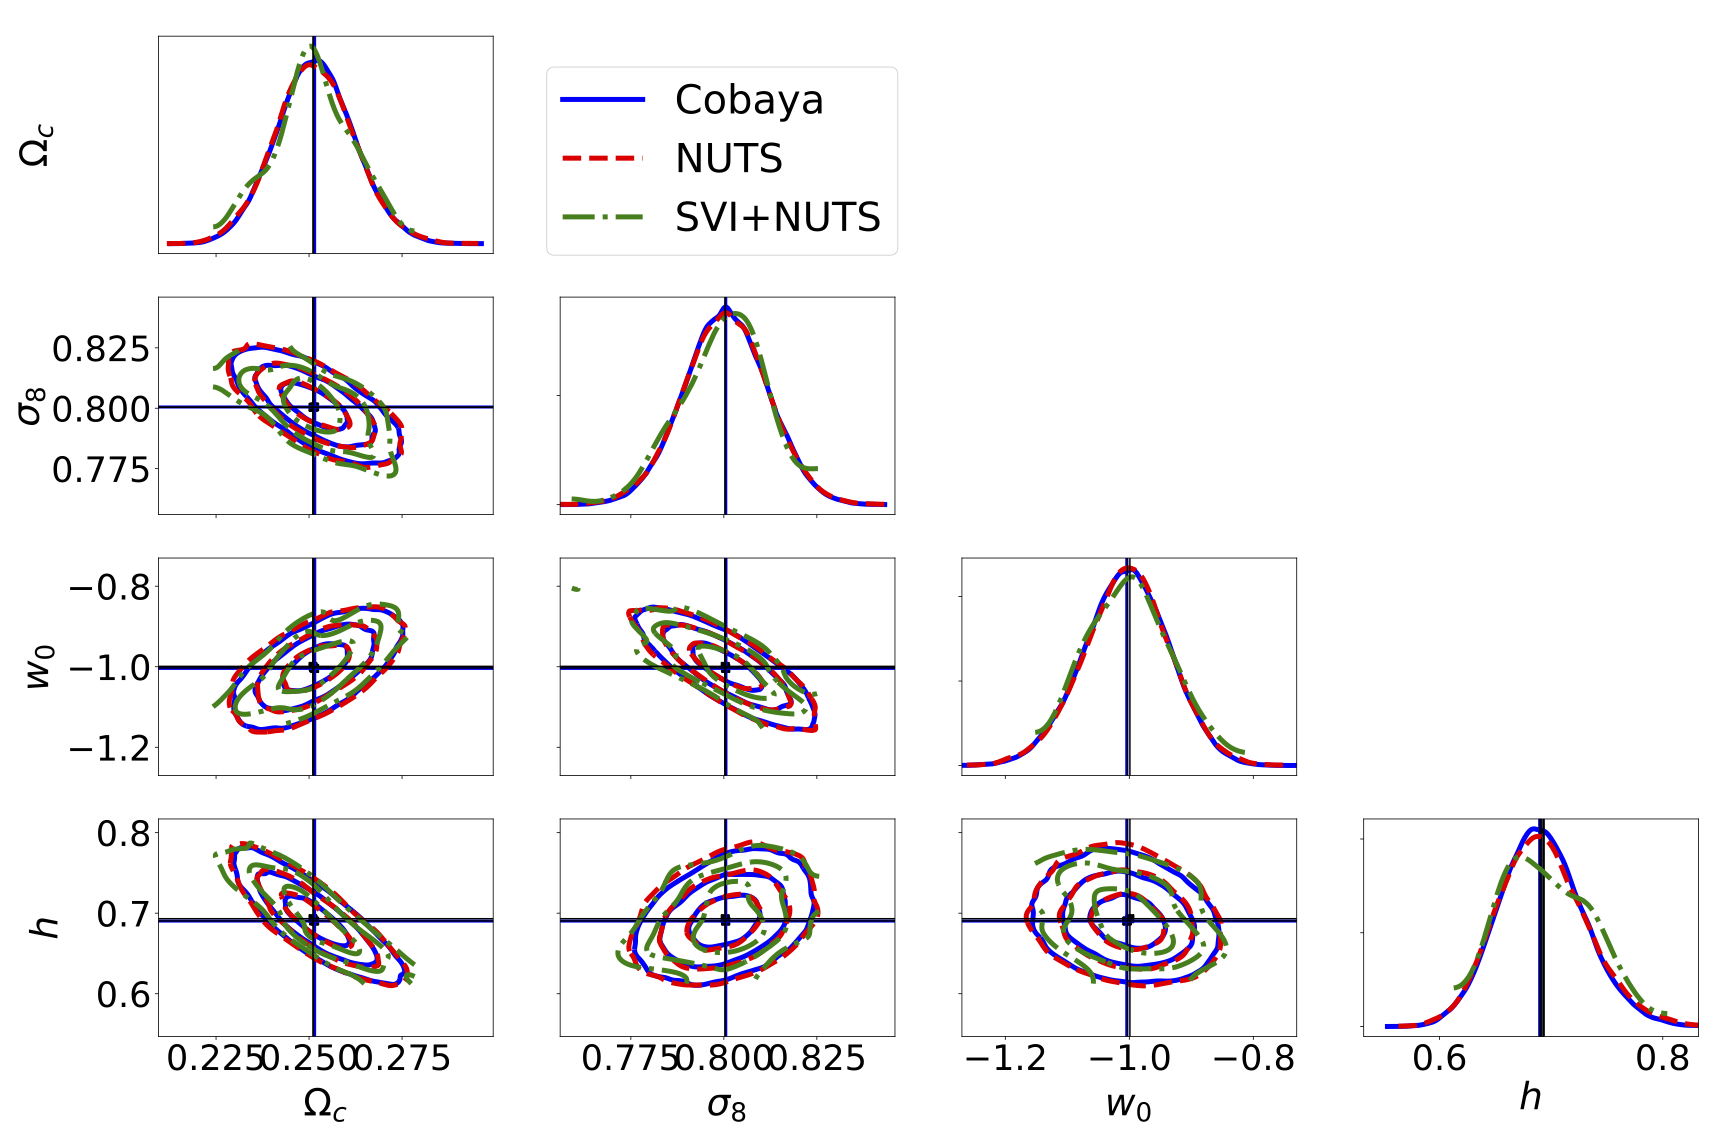
\includegraphics[width=1.5\columnwidth]{figures/Cobaya-NUTS-SVI200.png}
\caption{Constraints (30\%, 68\%, 90\%) on 4 of the 21 parameters of a simulated DES-Y1 3x2pt likelihood, using the \texttt{Cobaya} Metropolis-Hastings sampler (full curve in blue, 70,000 samples), the  NUTS sampling described in section \ref{sec-NUTS} (dashed curve in red; 16,000 samples), and a SVI MVN optimisation followed by a Naural Transport parametrisation to run a NUTS sampling (dashed-dotted curve in green, 200 samples).}
\label{fig_cobaya_NUTS_SVI}
\end{figure*}



\section{Application: Stochastic Variational Inference}
\label{sec-SVI}
%
Let us remind briefly what is the \textit{Stochastic Variational Inference} method \citep{2012arXiv1206.7051H, 2017arXiv171105597Z} and show where auto-differentiation helps. If one  writes $p(z)$ the prior, $p(\mathcal{D}|z)$ the likelihood and $p(\mathcal{D})$ the marginal likelihood, then thanks to the  Bayes theorem one gets $p(z|\mathcal{D})=p(z)p(\mathcal{D}|z)/p(\mathcal{D})$ the posterior distribution of a model with latent variables $z$ and a set of observations $\mathcal{D}$. The VI aims to get an approximation of this distribution, ie. $p(z|\mathcal{D}) \approx q(z;\lambda)$, by determining the variational parameters $\lambda$ of a predefined distribution. To do so, one uses the Kullback-Leibler divergence of the two distributions $KL(q(z;\lambda)||p(z|\mathcal{D}))$ leading to the following relation
\begin{align}
\log p(\mathcal{D}) &= \mathtt{ELBO} +  KL(q(z;\lambda)||p(z|\mathcal{D})) \label{eq-ELBO} \\
\mathrm{with} \ \mathtt{ELBO} &\equiv -\mathbb{E}_{q(z;\lambda)}\left[ \log q(z;\lambda)\right] + \mathbb{E}_{q(z;\lambda)}\left[ \log p(z,\mathcal{D}) \right] 
\end{align}
which defines the \textit{evidence lower bound} (aka ELBO) that one aims to maximize to get the $\lambda$ values. So, the optimal variational distribution satisfies
\begin{equation}
q(z;\lambda^\ast) = \underset{q(z;\lambda)}{\mathrm{argmax}}\  \mathtt{ELBO} = 
\underset{\lambda}{\mathrm{argmin}}\ \mathcal{L}(\lambda)
\end{equation}
The function $\mathcal{L}(\lambda)$ is the cost function used in practice. It is composed of two parts:
\begin{equation}
\mathcal{L}(\lambda) = \underbrace{\mathbb{E}_{q(z;\lambda)}\left[ \log q(z;\lambda)\right]}_{guide} - \underbrace{\mathbb{E}_{q(z;\lambda)}\left[ \log p(z,\mathcal{D}) \right]}_{model}
\label{eq-loss-svi-1}
\end{equation}
where the \textit{guide} in the \numpyro\ library may be a multi-variate Gaussian distribution (MVN) for instance.

Using the auto-differentation tool, one can use "black-box" guides (aka \textit{automatic differentiation variational inference}). As stated by the authors of \citep{2016arXiv160300788K} ADVI helps specifying a variational family appropriate to the model, computing the corresponding objective
function, taking derivatives, and running a gradient-based or coordinate-ascent optimization. First is defined a bijective differentiable transformation $T$ of the original latent variables $z$ into new variables $\xi$, such $\xi=T(z)$ and $z=T^{-1}(\xi)$. One can develop "AutoGuides" (\numpyro\ terminology) that can be adapted to the user models. Then, the cost function reads
\begin{equation}
\mathcal{L}(\lambda) = \underbrace{\mathbb{E}_{q(\xi;\lambda)}\left[ \log q(\xi;\lambda)\right]}_{guide} - \underbrace{\mathbb{E}_{q(\xi;\lambda)}\left[ \log p(\xi,\mathcal{D}) \right]}_{model}
\label{eq-loss-svi-2}
\end{equation}
with
\begin{equation}
p(\xi,\mathcal{D}) \bydef p(T^{-1}(\xi),\mathcal{D}) |J_{T^{-1}}(\xi)|
\end{equation}
which exhibit the Jacobian of the $T^{-1}$ transformation. The main advantage of this reparametrisation is that the minimization can be performed with no bound constraints. 

Now, one is faced with the evaluation of the expectations during gradient descent. The solution is to use what is called \textit{elliptical standardisation} or \textit{re-parametrization trick} or \textit{coordinate transformation} (see references in \citep{2015arXiv150603431K}). Let us illustrate the trick in the case where $q(\xi; \lambda) = \mathcal{N}(\xi; \mu, \Sigma)$ (ie. a MVN distribution with the parameters $\lambda=(\mu, \Sigma)$). One defines $S_\lambda$ such that $S_\lambda(\xi)=\zeta$, eg. $\zeta = L^{-1}(\xi-\mu)$ where $L$ is the Cholesky decomposition of $\Sigma=LL^T$. The Jacobian of this distribution is 1 (volume conservation), so the cost function reads
\begin{multline}
-\mathcal{L}(\lambda) = \underbrace{\mathbb{E}_{\zeta\sim \mathcal{N}(0,I)}\left[ \log p(T^{-1}(S_\lambda^{-1}(\zeta)),\mathcal{D}) + \log |J_{T^{-1}}(S_\lambda^{-1}(\zeta))| \right]}_{model} \\ + \underbrace{\mathbb{H}[q(\xi;\lambda)]}_{guide}
\label{eq-loss-svi-3}
\end{multline}
where $\mathbb{H}(q)$ is the Shannon entropy of the MVN distribution which is independent of the model, so its gradient can be computed once for all and reused in any user model. Then,
to get $\nabla_\lambda \mathcal{L}$, the $\nabla$ operator can be put inside the expectation which leads to\footnote{To simplify the notation, $T^{-1}(S_\lambda^{-1}(\zeta))$ has been replaced by $z$.}
\begin{multline}
-\nabla_\lambda\mathcal{L}(\lambda) = \mathbb{E}_{\zeta\sim \mathcal{N}(0,I)}\left\{
\left[ \nabla_z \log p(z,\mathcal{D}) \times \nabla_\xi[T^{-1}(\xi)] \right. \right. \\
+ \left. \left. \nabla_\xi \log|J_{T^{-1}}(\xi)| \right] \times \nabla_\lambda S_\lambda^{-1}(\zeta)
\right\}
+ \nabla_\lambda \mathbb{H}[q(\xi;\lambda)]
\label{eq-loss-svi-4}
\end{multline}
For the use case of the MVN (auto)guide, one gets
\begin{align}
-\nabla_\mu \mathcal{L} &= \mathbb{E}_{\zeta\sim \mathcal{N}(0,I)}\left\{
\nabla_z \log p(z,\mathcal{D}) \times \nabla_\xi[T^{-1}(\xi)]
+ \nabla_\xi \log|J_{T^{-1}}(\xi)|
\right\} \nn \\
-\nabla_L \mathcal{L} &= \mathbb{E}_{\zeta\sim \mathcal{N}(0,I)}\left\{
\left[ \nabla_z \log p(z,\mathcal{D}) \times \nabla_\xi[T^{-1}(\xi)] \right.\right. \nn\\
&\left. \left. \qquad\qquad\qquad + \nabla_\xi \log|J_{T^{-1}}(\xi)| \right] \times \xi^T 
\right\}+ (L^{-1})^T
\end{align}
The expectations used in the above expressions are computed with $\zeta$ i.i.d samples from $\mathcal{N}(0,1)$ distribution which reveals the "S" of SVI. As one can imagine all the jacobian computations take benefit of the automatic differentiation offers by JAX. Now even if one can sample from the optimized  $q(z,\lambda^\ast)$ distribution, we have used SVI as front-end to a NUTS sampler which is described in the next section \ref{sec-Neural-Reparametrisation} and nicknamed as \textit{Neural Transport}.
%
\subsection{Neural Transport}
\label{sec-Neural-Reparametrisation}
%
If the SVI method can be used as is to get $z$ i.i.d. samples from the $q(z,\lambda^\ast)$ distribution, the \textit{Neural Transport MCMC} method \citep{2014arXiv1412.5492P,2019arXiv190303704H} is an efficient way to boost HMC efficiency, especially in target distribution unfavourable geometry where for instance the leapfrog integration algorithm has to face squeezed join distributions for a subset of variables. From SVI, one obtains a first approximation of the target distribution and we show that the change-of-variable $z=F_\lambda(\zeta)$ is such that
\begin{equation}
q(z;\lambda) \rightarrow q(\zeta;\lambda) \bydef q(F_\lambda(\zeta)) |J_{F_\lambda}(\zeta)|
\end{equation}
which is evaluated with optimal $\lambda^\ast$ according to maximization of the ELBO (eg. $F_\lambda=T^{-1}\circ S^{-1}_\lambda$). So, one can use a HMC sampler (eg. NUTS) based on $p(\zeta;\mathcal{D})$ distribution, initialized with $\zeta$ samples from $q(\zeta;\lambda^\ast)$, to get a Markov Chain of $N$ samples $(\zeta_i)_{i<N}$. Then, from the transformation  $z_i=F_{\lambda^\ast}(\zeta_i)$ one finally obtain a Marcov Chain with $(z_i)_{i<N}$ samples. The method is accessible throw the \verb|NeuTraReparam| in \numpyro\ library.

%\begin{figure}
%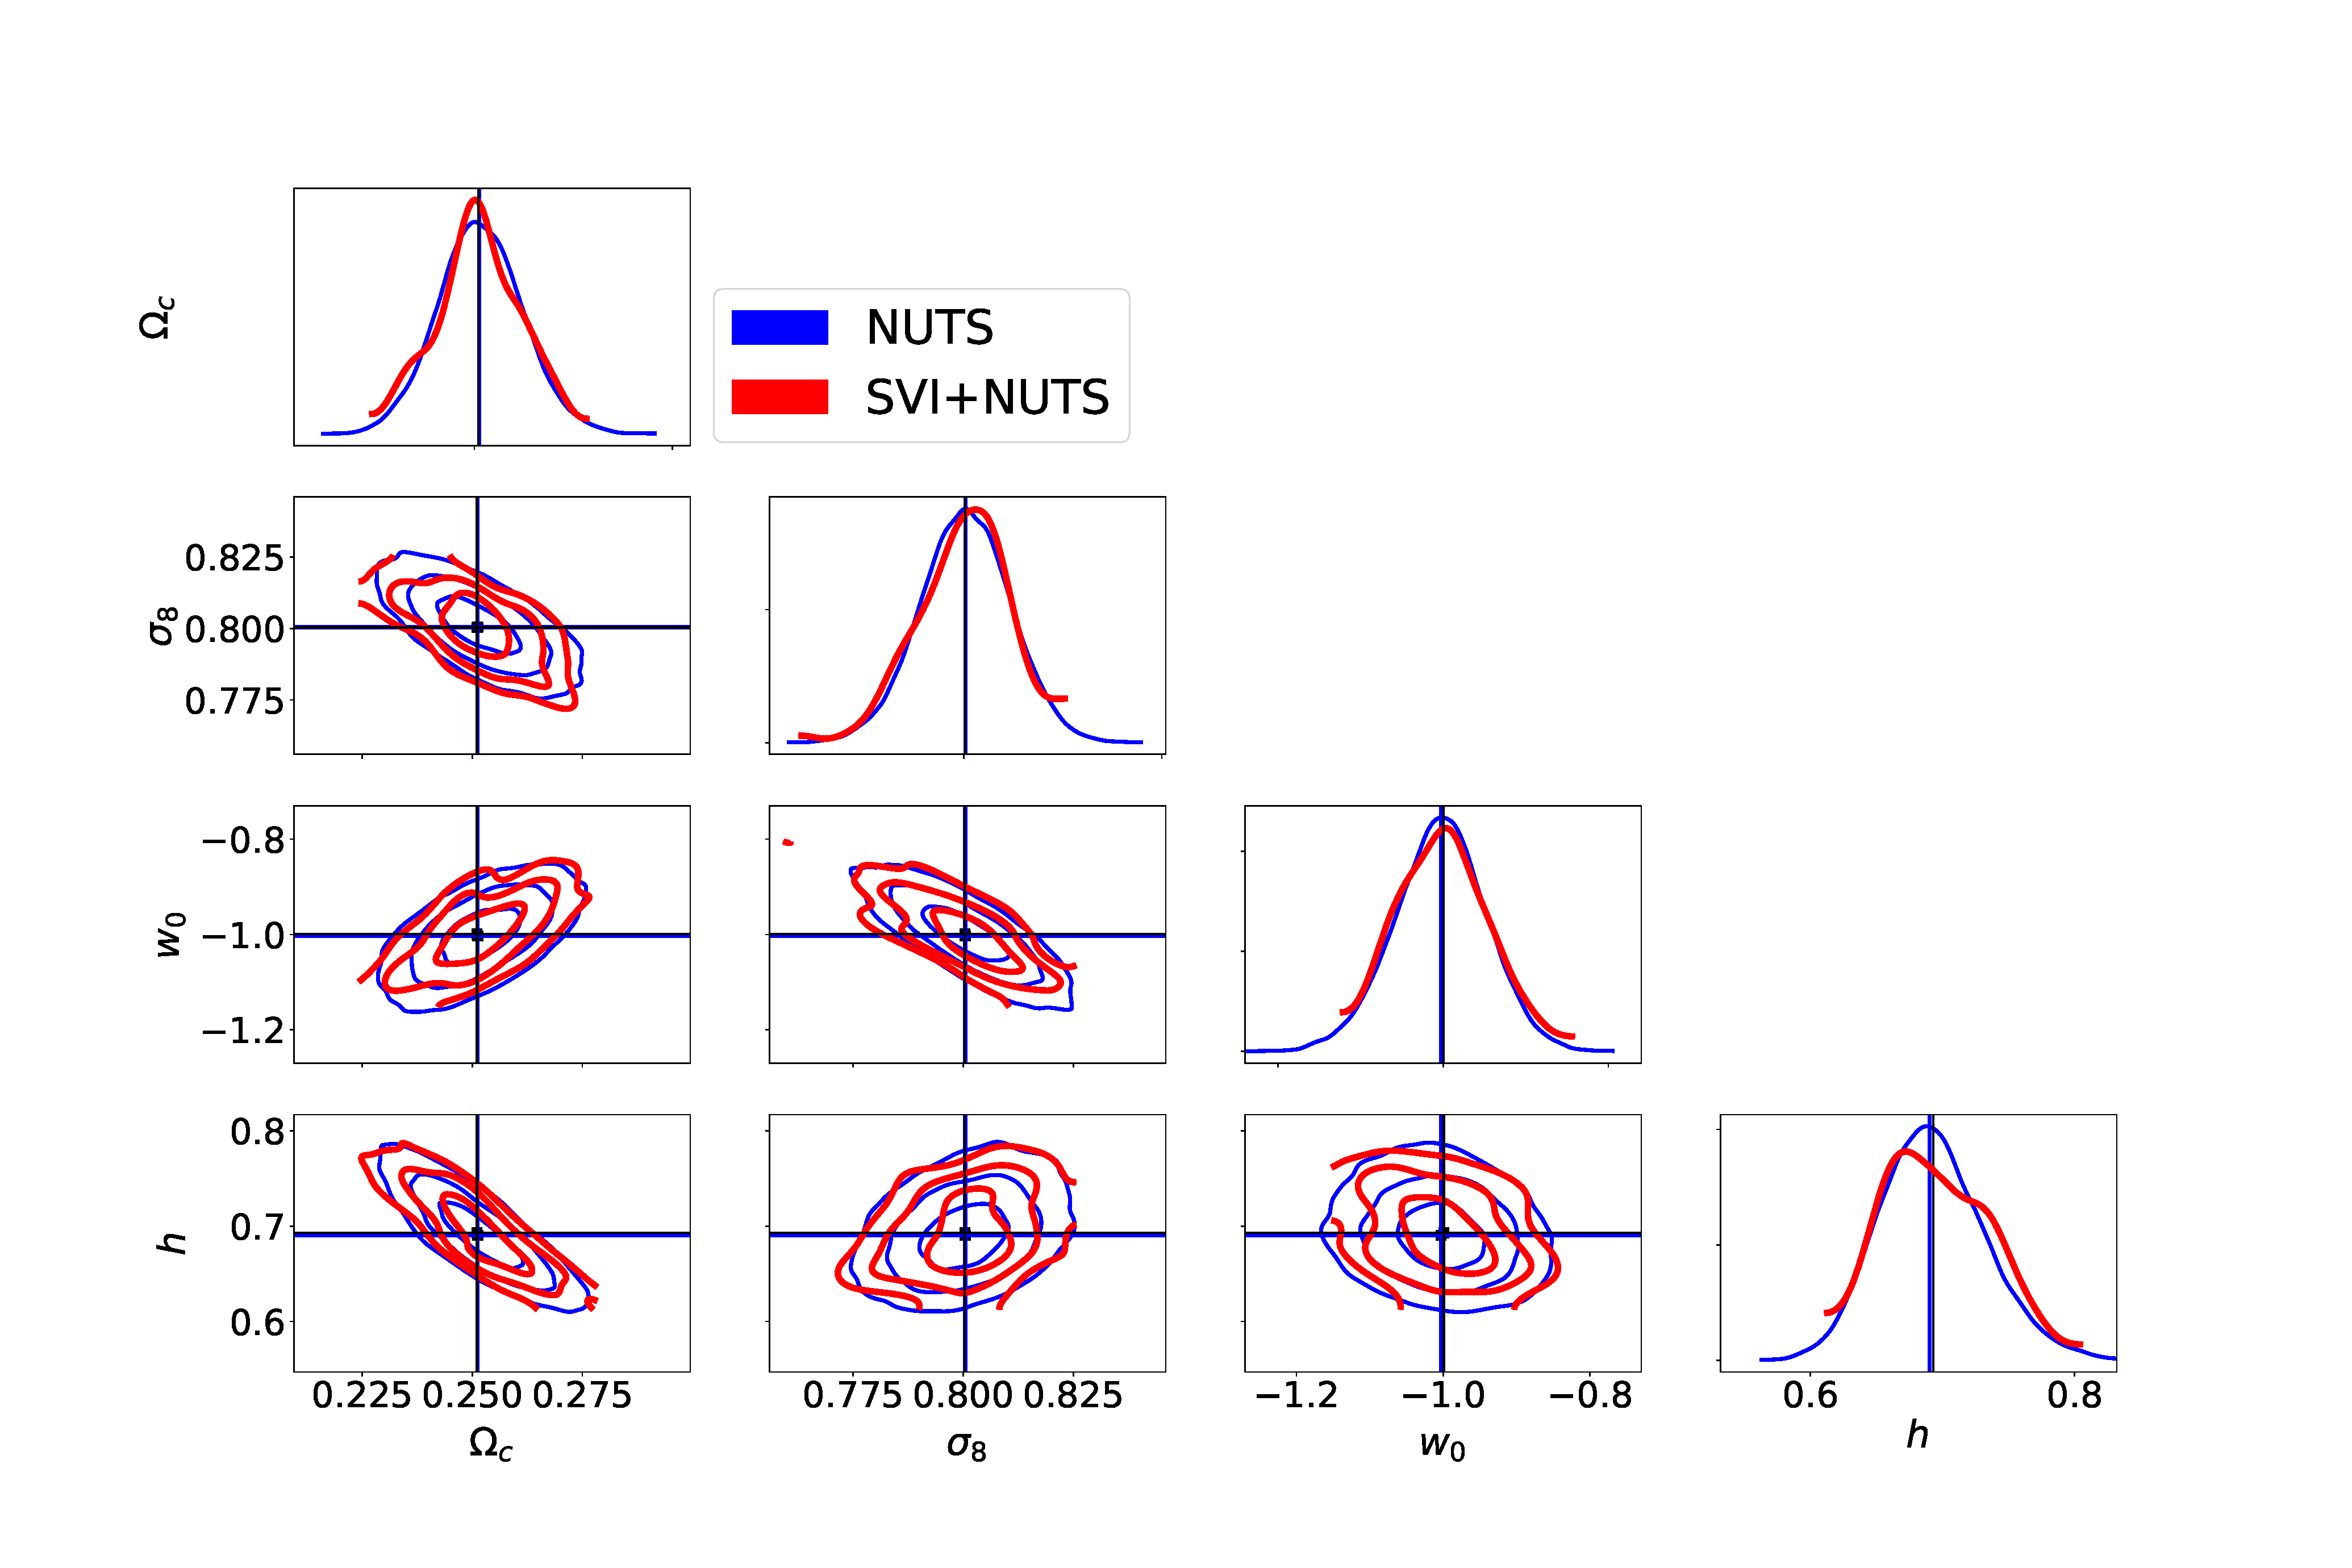
\includegraphics[width=\columnwidth]{figures/SVI_NUTS_1x200x200.pdf}
%\caption{Constraints (30\%, 68\%, 90\%) on 4 of the 22 parameters of a simulated DES-Y1 3x2pt likelihood, in blue the NUTS sampling described in section \ref{sec-NUTS}, and in orange a SVI MVN optimisation followed by a Naural Transport parametrisation to run a NUTS sampling (1 chain of 200 warm followed by 200 samples; a dense mass matrix and \texttt{max\_tree\_depth} parameter set to 5).}
%\label{fig_svi_nuts_1}
%\end{figure}

%\begin{figure}
%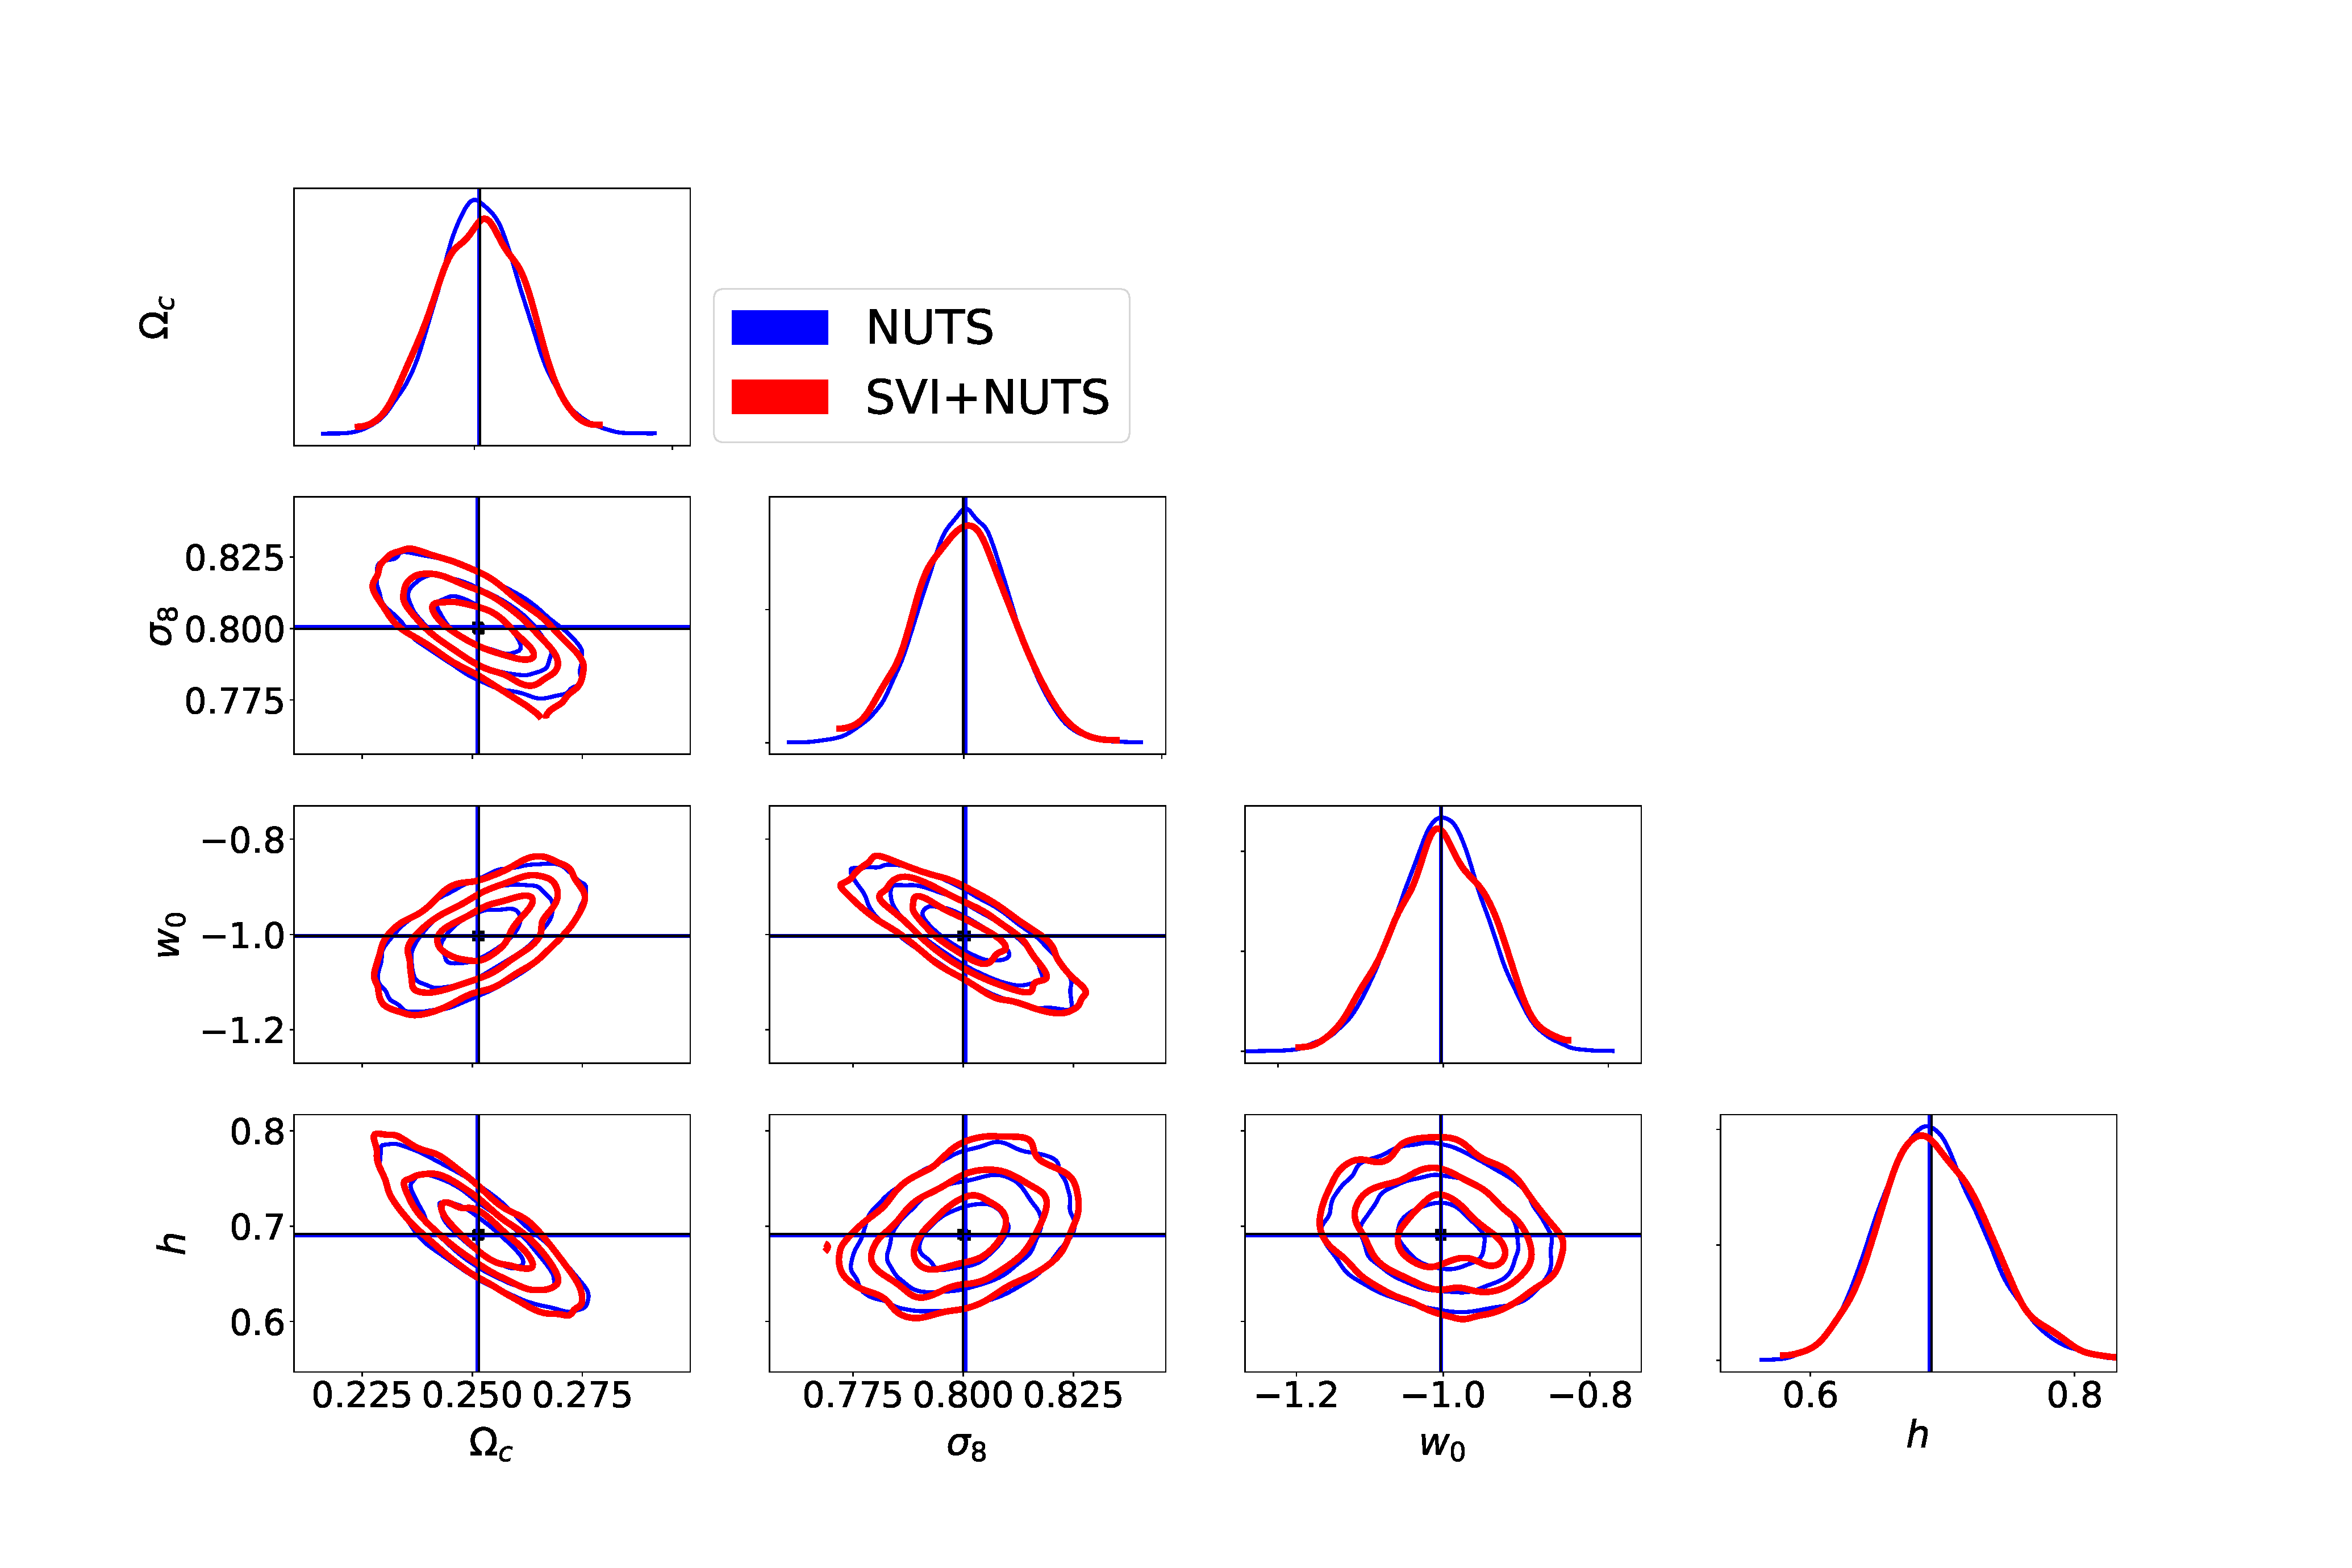
\includegraphics[width=\columnwidth]{figures/SVI_NUTS_1x200x1000.pdf}
%\caption{Same as Fig.~\ref{fig_svi_nuts_1} but with 1 chain of 200 warm followed by 1000 samples for the NUTS sampler after SVI optimization.}
%\label{fig_svi_nuts_2}
%\end{figure}
%
%\begin{figure}
%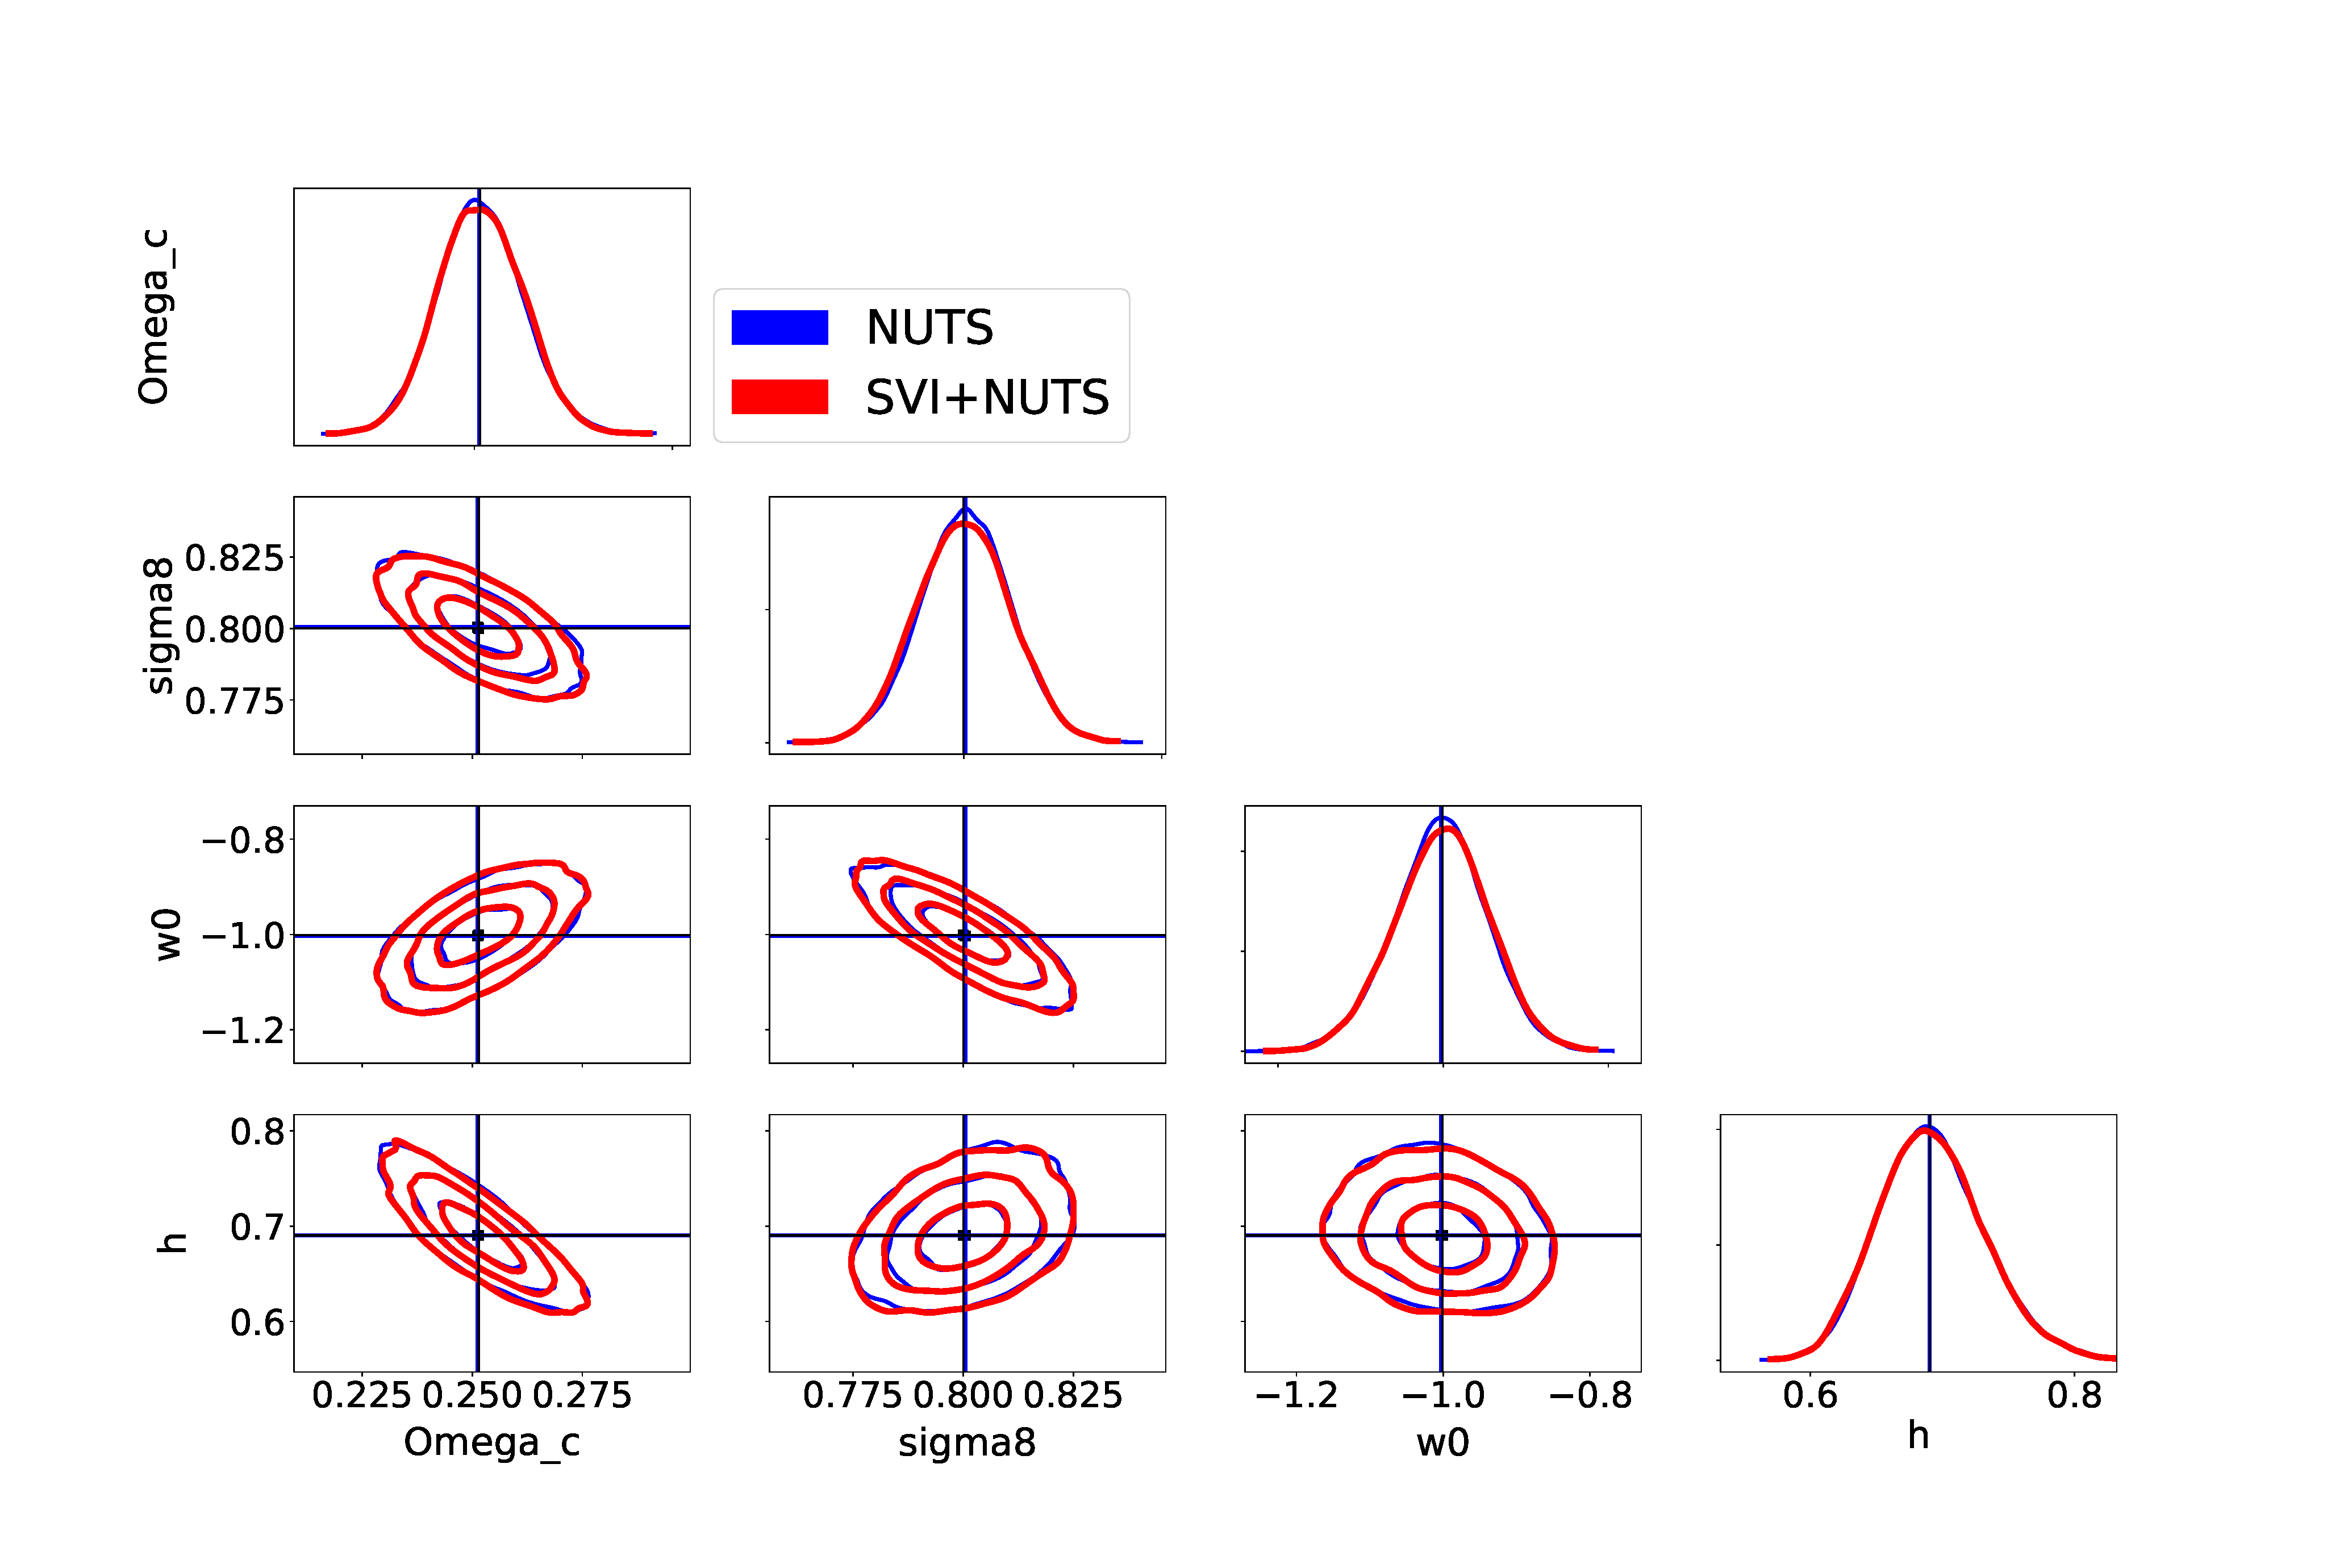
\includegraphics[width=\columnwidth]{figures/SVI_NUTS_10x200x1000.pdf}
%\caption{Same as Fig.~\ref{fig_svi_nuts_1} but with 10 chains of 200 warm followed by 1000 samples for the NUTS sampler (\texttt{max\_tree\_depth=5}) after SVI optimization.}
%\label{fig_svi_nuts_3}
%\end{figure}

%\begin{figure}
%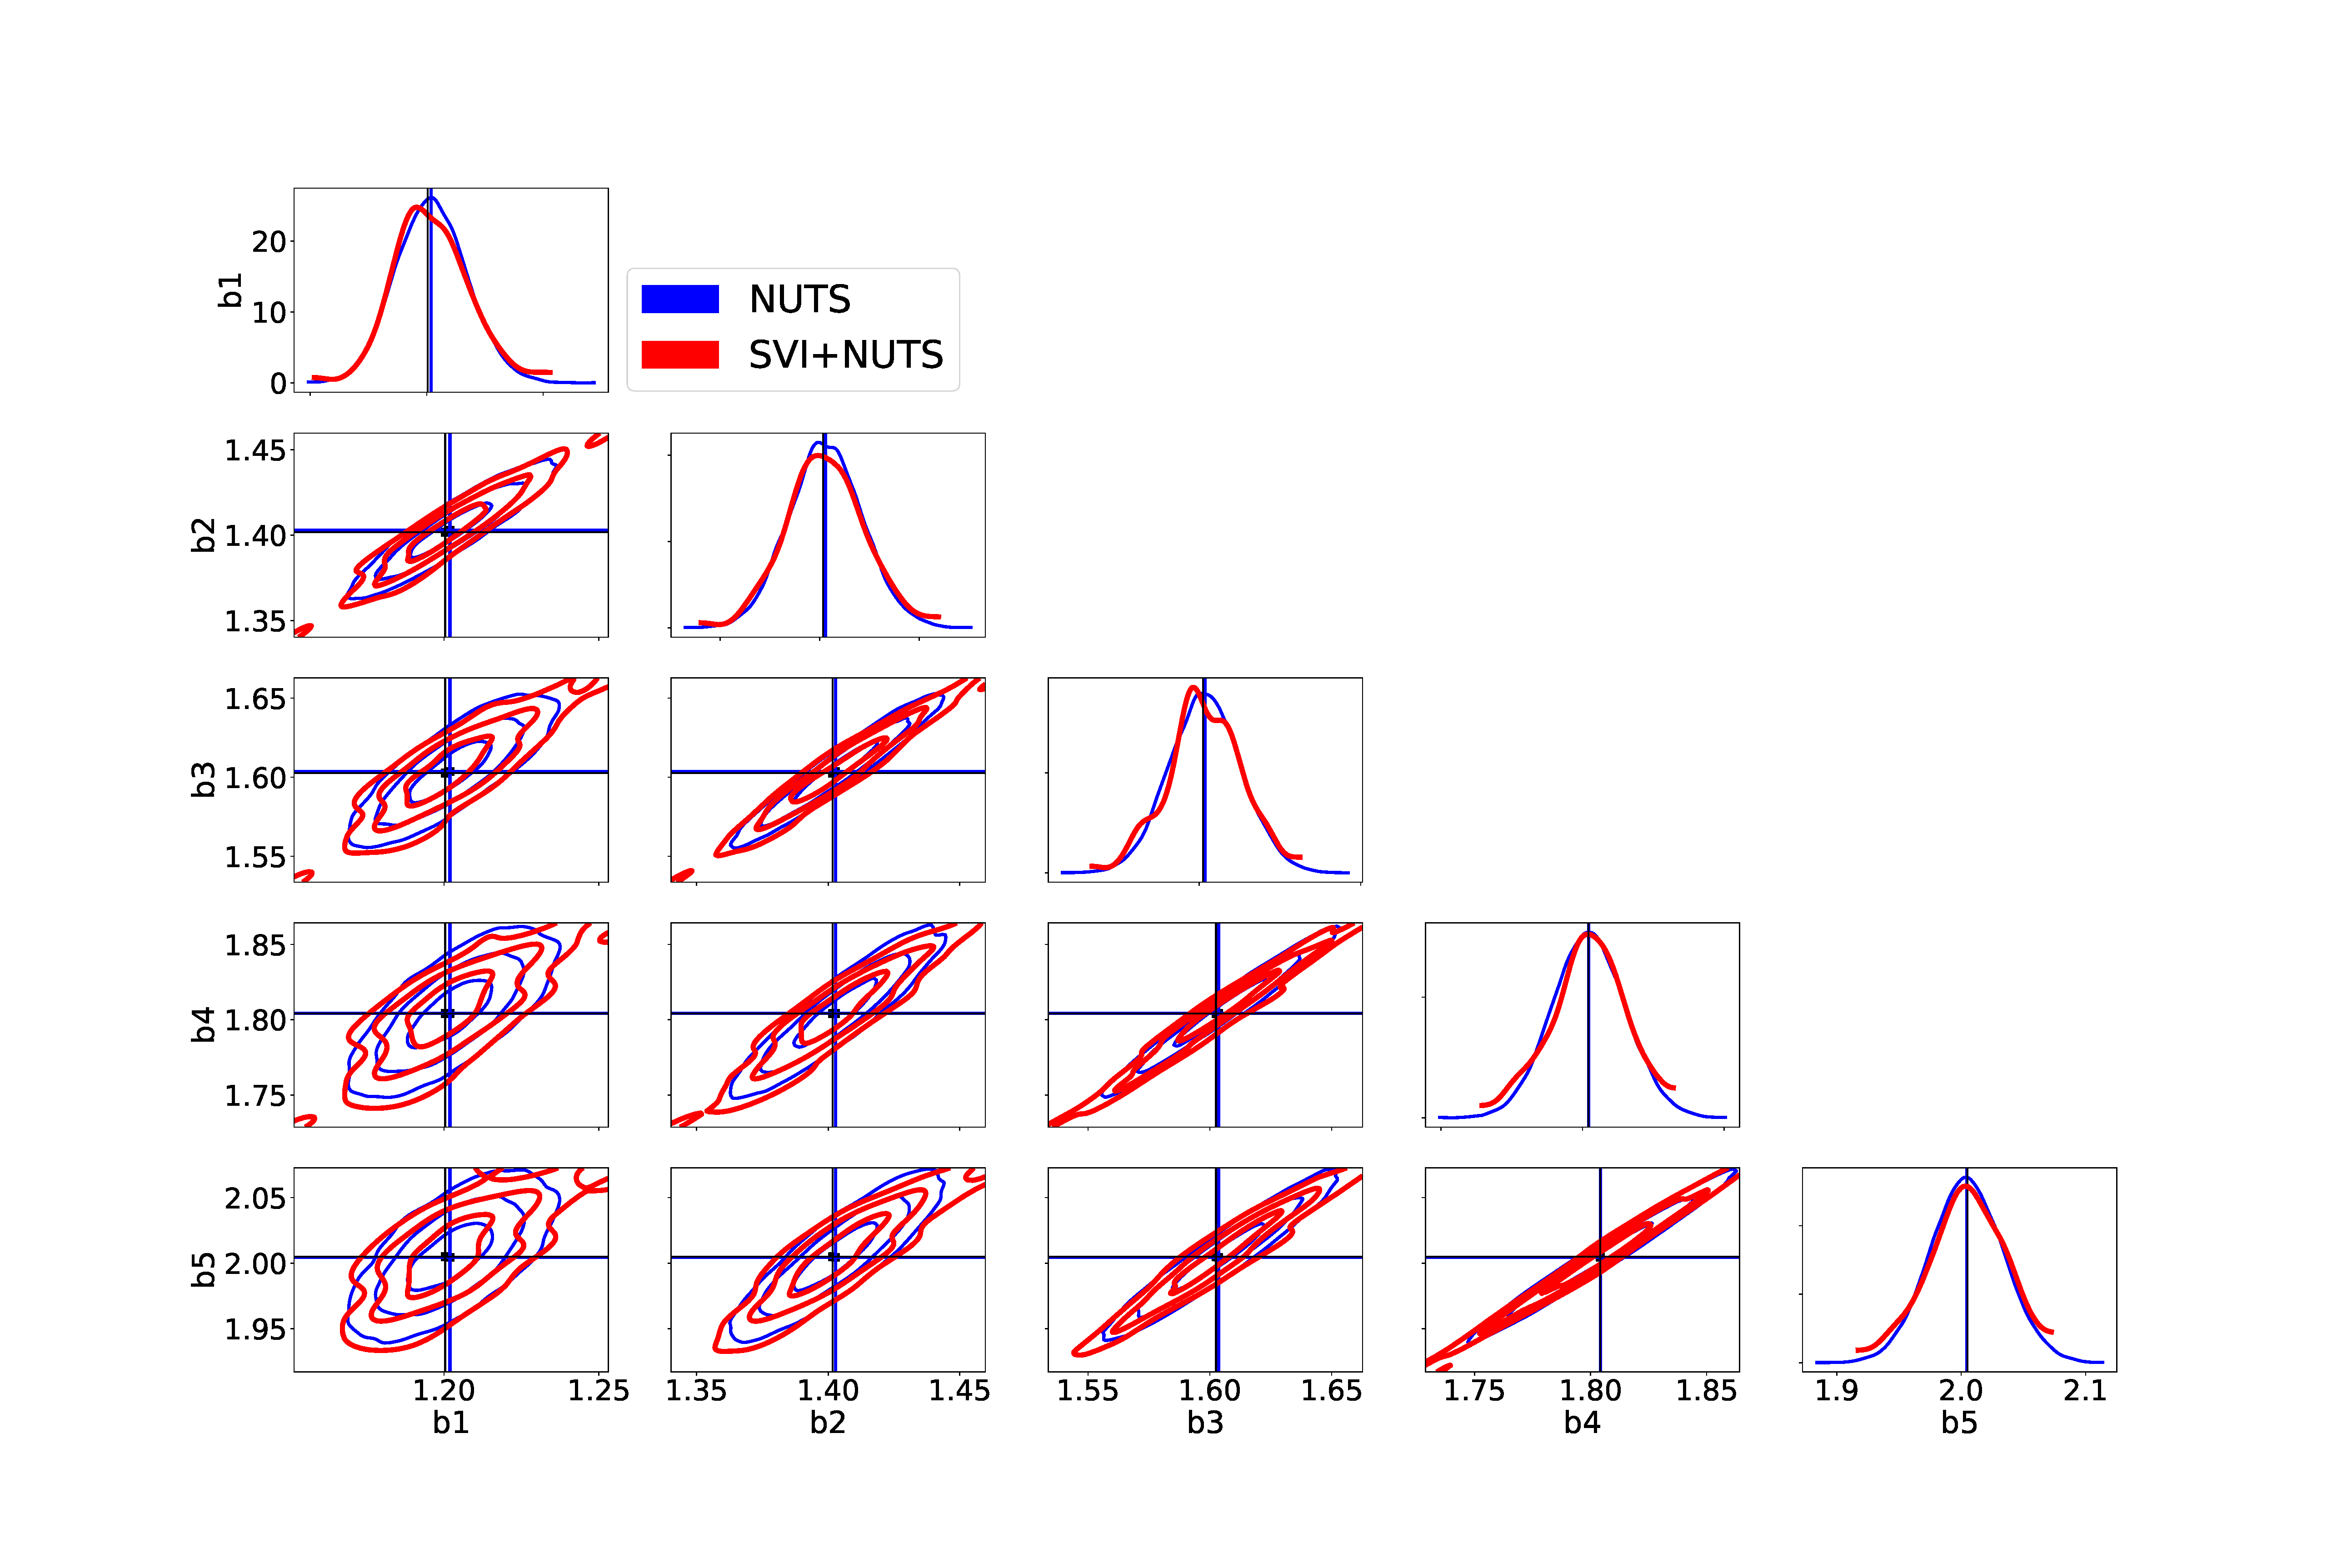
\includegraphics[width=\columnwidth]{figures/SVI_NUTS_1x200x200_bis.pdf}
%\caption{
%Constraints (30\%, 68\%, 90\%) on the five lens galaxy bias. In blue the NUTS sampling described in section \ref{sec-NUTS}, and in red a SVI MVN optimisation followed by a Naural Transport parametrisation to run a NUTS sampling (1 chain of 200 warm followed by 200 samples; a dense mass matrix and \texttt{max\_tree\_depth} parameter set to 5).}
%\label{fig_svi_nuts_4}
%\end{figure}

\begin{figure}
\centering
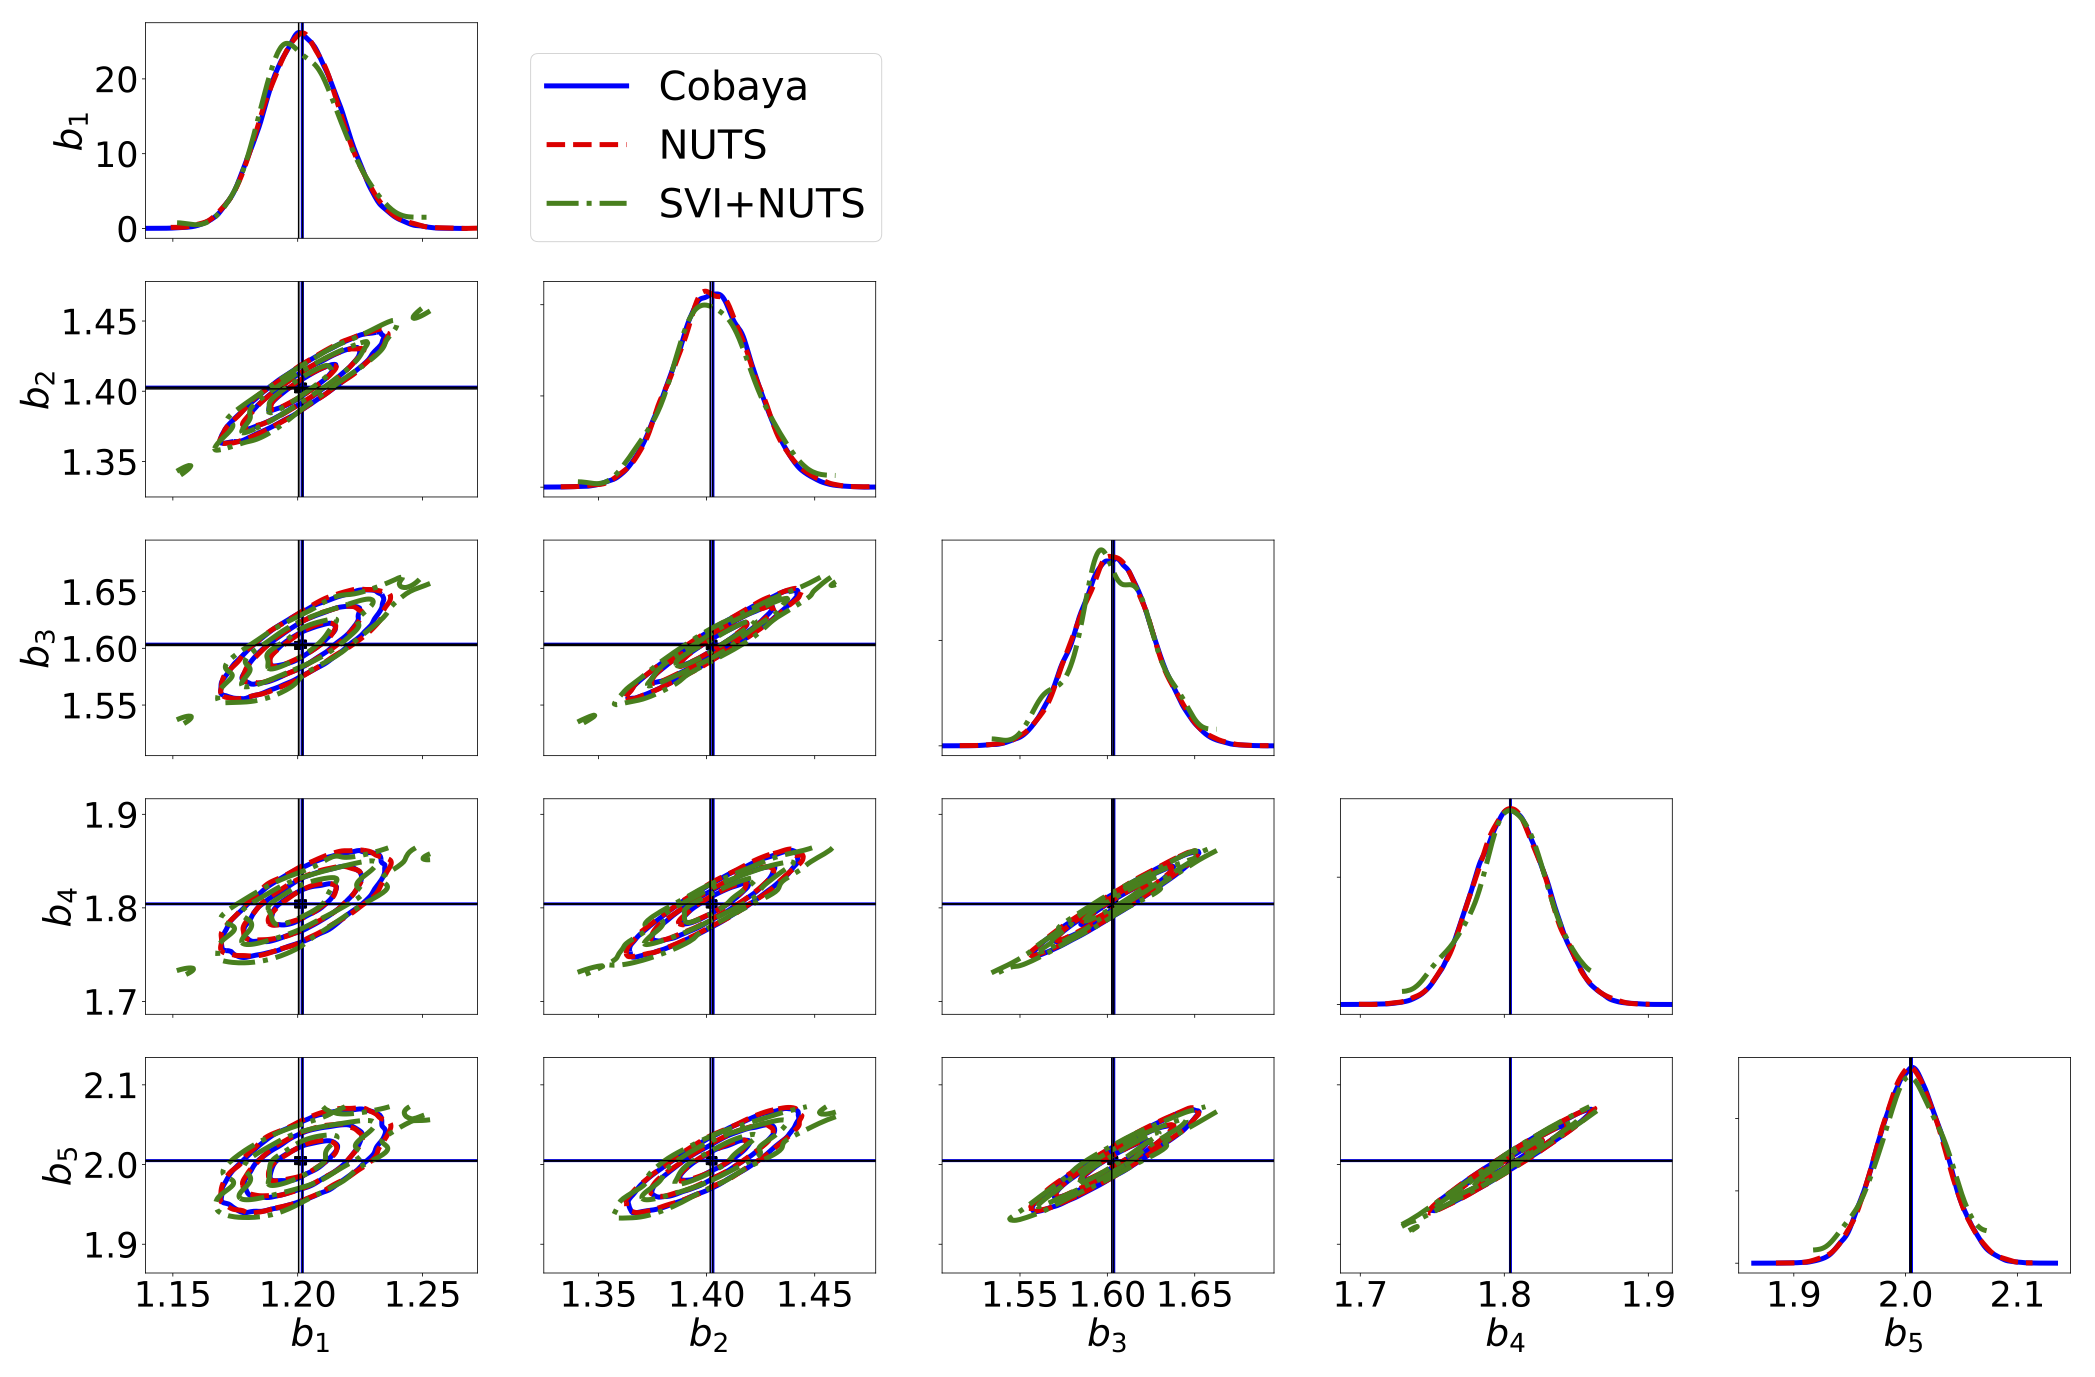
\includegraphics[width=\columnwidth]{figures/Cobaya-NUTS-SVI200_bis.png}
\caption{Same configuration as in Figure \ref{fig_cobaya_NUTS_SVI} but for the highly correlated five lens galaxy bias.}
\label{fig_cobaya_NUTS_SVI_bis}
\end{figure}


Using the same DES-Y1 simulation as in previous section, we use a MVN distribution as \textit{guide} to approximate the true posterior (\textit{model}) and feed a SVI. The SVI optimization has been performed with the Adam optimizer \citep{2014arXiv1412.6980K} and a learning rate set to $10^{-3}$. We have stopped the optimization after 20,000 steps to ensure a good convergence of the ELBO loss, but no particular tuning of the optimizer has been undertaken to decrease the number of steps. It takes 2 hours on the NVidia V100 GPU.  

Then, we have used the Neural Transport method to generate Markov Chains of different sizes by the NUTS sampler, the chains have run 200 warm samples, and then 200 samples ("low" schema), 1000 samples on a single chain, and finally we have run 10 chains  with 1000 samples each. All NUTS sampling as been performed with dense mass matrix optimisation without special block structuring and with \texttt{max\_tree\_depth=5} which is different than the default NUTS setting described in section \ref{sec-NUTS}. The elapse time for each of these 3 runs is 50 minutes, 150 minutes and 5 hours, respectively. Naturally, more samples lead to better contour precision. But what is illustrative is the "low" schema results as shown in the Figures \ref{fig_cobaya_NUTS_SVI} and \ref{fig_cobaya_NUTS_SVI_bis}  to be compared to \texttt{Cobaya} and NUTS results presented in section \ref{sec-NUTS}. Notice the good results even for the highly correlated lens bias parameters. It is noticeable that running NUTS with the same settings  but without the SVI Neural Transport phase has demonstrated a rather poor behaviour with only 200 samples.  

Results in terms of sampling efficiency are shown on Table~\ref{tab-ESS-NUTS_SVI-1} showing that the SVI followed by Neutral Transport gives high efficiency at low number of samples which is quite interesting to ease the model development in its early phase.
%
\section{Discussion}
\label{sec-discussion}
%
To a large extend looking at results of Table~\ref{tab-ESS-NUTS_SVI-1}, the key question is: what is the HMC/NUTS gain compared to the well known highly optimized \texttt{Cobaya} sampler? 
In one hand, one may argue considering the elapse time of execution that the number of efficient samples per model call is a right metric to consider: 
\begin{equation}
    \eta = \frac{n_{eff}}{\#\ of\ calls} = \frac{N_s \times \varepsilon}{N_s \times n_{steps}} = \frac{\varepsilon}{n_{steps}}
\end{equation}
with $N_s$ the total number of samples, $\varepsilon$ the effective sampler efficiency  and $n_{steps}$ the number of steps (calls) per sample generation. Then, for \texttt{Cobaya} one roughly gets $\varepsilon\approx 3\%$ with $n_{steps}=1$ while for the NUTS sampler $\varepsilon\approx 50\%$ but at the expense of $n_{steps}=2^5$ or more. At the end of the day after tuning generation parameters, the $\eta$ values for both methods would certainly be comparable (ie. about $1\%$). So, at first sight one may conclude that there is no gain to use HMC/NUTS compared to standard MCMC sampler.  

On the other hand, the above metric is may be too crude to cover all aspects of the sample generation. One should probably have in mind that the low sampling efficiency of standard MCMC sampler requires mobilizing a large amount of resources to produce a sufficient large sample batch in a reasonable time scale, ie. several days on dedicated infrastructure. Moreover, the user is faced to the dilemma to perform or not a statistical sample selection post-processing as \textit{thinning} beyond the \textit{burn-in removal} which is a rather delicate procedure and time consuming too, needing how-know to be conducted correctly \citep{doi:10.1146/annurev-statistics-040220-091727, 2015arXiv151007727O}. 

So, the authors think that it is worth considering methods like HMC/NUTS that by construction are more efficient. Moreover, using SVI with neural reparametrisation offers an effective way to undertake a progressive validation of the model with rather modest sample set (eg. starting with 200 samples) producing good enough marginal contours in few hours. In practice, this validation phase can save time before producing sizeable batch for final analysis. The authors have not investigated very high dimensional ($O(10^2)$ parameters) as well as multi-modal analysis, but the key argument in favour of HMC/NUTS sampling is that it exploit the geometry of the typical set of the posterior distribution contrary to the standard random walk of Metropolis-Hasting sampling. Furthermore, using reparametrisation  one can adapt to poor geometry cases (eg. \cite{2019arXiv190303704H}).
%
\begin{table}[htb]
\caption{Results of the \textit{relative effective sample size} (aka ESS, "bulk") in percent computed by the \texttt{Arviz} library \citep{arviz_2019}. The ESS can be larger than 100\% in some cases. 
%{\color{red} 
%(0) "F.L run" are computed from NUTS sampler with 16 %parallel chains of 1,000 samples each and 200 warm-up %and \texttt{max\_tree\_depth=7} (see text) The numbers %are from \texttt{n\_eff/16,000};
%}
(a): results from Cobaya 70,000 samples;
(b): results from NUTS sampler with 16 chains of 1,000 samples each and 200 warm-up and \texttt{max\_tree\_depth=7} (Section~\ref{sec-NUTS}); 
(c) are the results of SVI Multivariate Normal followed by NUTS and Neural Transform  with 1 chain of 200 samples and 200 warm-up (Section~\ref{sec-Neural-Reparametrisation}).}
\label{tab-ESS-NUTS_SVI-1}
 \centering
\begin{tabular}{ccccccccccc}
\hline
    & $\Omega_b$ & $\Omega_c$ & $\sigma_8$ & $w_0$ & $h$ & $n_s$ & $A$ & $\eta$\\
\hline
(a) &  $3.1$ & $2.5$       & $2.9$      & $2.9$  & $2.6$  & $3.1$  & $3.1$ & $2.8$ \\  
(b) & $48.1$ &  $45.6$     & $36.2$     & $33.4$ & $52.8$ & $50.1$ & $68.8$ & $48.8$\\
(c) & $84.0$ &  $28.0$     & $26.0$     & $20.5$ & $80.0$ & $110.5$ & $58.5$ & $29.5$\\
\hline
\end{tabular}
\end{table}


\section{Conclusions \& Prospects}
\label{sec-conclusion}

\FrL{mention something about scaling with parallel MCMC}

\subsection{Efficient sampling in high dimensions with Hamiltonian Monte Carlo}



\subsection{Lightning fast inference with BayesFast}

%
%
\subsection{DES-Y1 Example}
%

%%%
\section*{CRediT authorship contribution statement}
\textbf{J.E Campagne} Conceptualization, Methodology, Software, Validation, Writing.
\textbf{F. Lanusse}, \textbf{J. Zuntz}...

%\section*{Declaration of Competing Interest}
%The authors declare that they have no known competing financial interests or personal relationships that could have appeared to influence the work reported in this paper.

%\Acknowledgements
\section*{Acknowledgements}
Some of the numerical experiments have been conducted at the IN2P3 Computing Center (CC-IN2P3 - Lyon/Villeurbanne - France) funded by the Centre National de la Recherche Scientifique.


%% The Appendices part is started with the command \appendix;
%% appendix sections are then done as normal sections
\appendix

\section{Description of the DES-Y1 exercise}
\label{app-DESY1}
From the DES server\footnote{\url{http://desdr-server.ncsa.illinois.edu/despublic/y1a1_files/chains/2pt_NG_mcal_1110.fit}} we have extracted the $N(z)$ distributions of the sources and normalize them to $[1.47, 1.46, 1.50, 0.73]$ effective number of sources per $\mathrm{arcmin}^2$ for each of the four redshift bins, respectively. The lens distributions $N(z)$ for five redshift bins are also extracted. The corresponding shapes of the different distributions are performed thanks to \texttt{jc.redshift.kde\_nz} function ("\texttt{jc}" hereafter stands for \texttt{jax\_cosmo}) and are presented in Figure \ref{fig-DESY1-src-lens-redshift}.
\begin{figure}
\centering
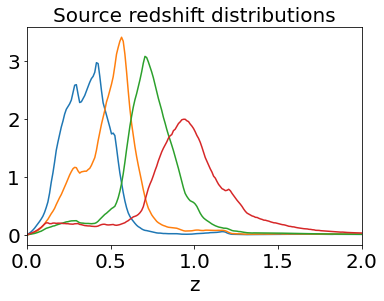
\includegraphics[height=3cm]{figures/DESY1-source-redshift.png}
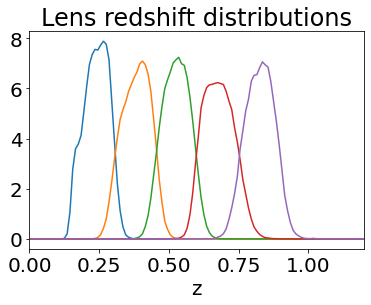
\includegraphics[height=3cm]{figures/DESY1-lens-redshift.png}
\caption{Distributions of the sources and lenses for the different redshift bins considered.}
\label{fig-DESY1-src-lens-redshift}
\end{figure}
\begin{table}[htb]
\caption{Priors of the 21 variables of the DES-Y1 of the 3x2pt likelihood (number counts and shear).}
\label{tab-DESY1}
 \centering
\begin{tabular}{ccccccccccc}
\hline
 parameter &  prior \\
 \hline
  \multicolumn{2}{c}{\textbf{Cosmology}} \\
$\Omega_b$ & $\mathcal{U}[0.10, 0.9]$ \\
$\Omega_c$ & $\mathcal{U}[0.40, 1.0]$ \\
$\sigma_8$ & $\mathcal{U}[0.03, 0.07]$ \\
$w_0$ & $\mathcal{U}[-2.00, -0.33]$ \\
$h$ & $\mathcal{U}[0.55, 0.91]$ \\
$n_s$ & $\mathcal{U}[0.87, 1.07]$ \\
\multicolumn{2}{c}{\textbf{Intrinsic Alignment}} \\
$A$ & $\mathcal{U}[-5,5]$ \\
$\eta$ &$\mathcal{U}[-5,5]$ \\
\multicolumn{2}{c}{\textbf{Lens Galaxy Bias}} \\
$(b_i)_{i:1,\dots,5}$ & $\mathcal{U}[0.8,3.0]$ \\
\multicolumn{2}{c}{\textbf{Shear Calibration Systematics}} \\
$(m_i)_{i:1,\dots,4}$ & $\mathcal{N}[0.012,0.023]$ \\
\multicolumn{2}{c}{\textbf{Source photo-$z$ shift}} \\
$dz_1$ & $\mathcal{N}[0.001,0.016]$ \\
$dz_2$ & $\mathcal{N}[-0.019,0.013]$ \\
$dz_3$ & $\mathcal{N}[0.009,0.011]$ \\
$dz_4$ & $\mathcal{N}[-0.018,0.022]$ \\
\hline
\end{tabular}
\end{table}


Then, using the \numpyro\ PPL, we have set up a \textit{forward model} following the reference \citep{2018PhRvD..98d3526A}. The prior descriptions of the different model parameters are described in Table \ref{tab-DESY1}.  For instance the $\Omega_c$ parameter is treated as random variable as followed
%\begin{minted}[fontsize=\footnotesize]{python}
\begin{lstlisting}[language=iPython]
Omega_c = numpyro.sample('Omega_c', Uniform(0.1, 0.9))
\end{lstlisting}
%\end{minted}

Then, we generate mock angular power spectra $C_\ell$ from the auto \& cross correlations of the Number Counts and Weak Lensing probes computed with the \texttt{gaussian\_cl\_covariance\_and\_mean} function in the \texttt{jc.angular\_cl} module. One reads
%\begin{minted}[fontsize=\footnotesize]{python}
\begin{lstlisting}[language=iPython]
# Define the lensing and number counts probe
probes = [jc.probes.WeakLensing(nzs_s_sys, 
                       ia_bias=b_ia,
                       multiplicative_bias=m),
          jc.probes.NumberCounts(nzs_l, b)]
cl, C = gaussian_cl_covariance_and_mean(cosmo, 
                 ell, probes, 
                 f_sky=0.25, sparse=True)
\end{lstlisting}
%\end{minted} 
with \texttt{cosmo} an instance of the \texttt{jc.Cosmology} setting the cosmological parameters generated with the priors, and \texttt{ell} (ie. $\ell$) a series of 50 angular modes. The generation of the mock data yields from the possibility to execute a conditioned model with a fiducial cosmology, leaving \numpyro\ dealing with the random number generation:
%\begin{minted}[fontsize=\footnotesize]{python}
\begin{lstlisting}[language=iPython]
fiducial_model = condition(model,
    {'Omega_c':0.2545, 'sigma8':0.801, 
    'h':0.682, 'Omega_b':0.0485, 'w0':-1.,'n_s':0.971,
     'A':0.5,'eta':0.,
     'm1':0.0,'m2':0.0,'m3':0.0,'m4':0.0,
     'dz1':0.0,'dz2':0.0,'dz3':0.0,'dz4':0.0,
     'b1':1.2,'b2':1.4,'b3':1.6,'b4':1.8,'b5':2.0
      })

with seed(rng_seed=42):
    data, P, C = fiducial_model()
\end{lstlisting}
%\end{minted}

The \textit{inference model} looks very similar to the \textit{forward model} excepts that first we fix the angular power spectra covariance matrix $C$ (and its inverse $P$) and secondly we let \numpyro\ generates the model $C_{\ell}$ from the priors
%\begin{minted}[fontsize=\footnotesize]{python}
\begin{lstlisting}[language=iPython]
cl = jc.angular_cl.angular_cl(cosmo, ell, 
                              probes).flatten()
return numpyro.sample('cl', MultivariateNormal(cl, 
                            precision_matrix=P,
                            covariance_matrix=C))
\end{lstlisting}
%\end{minted}

These theoretical $C_{\ell}$ are in turn conditioned by the mock $C_\ell$ as followed
%\begin{minted}[fontsize=\footnotesize]{python}
\begin{lstlisting}[language=iPython]
observed_model = condition(model, {'cl': data})
\end{lstlisting}
%\end{minted}
Then, as an example the optimisation of the cosmological parameters using for instance the NUTS flavour of MCMC can be conducted as followed
%\begin{minted}[fontsize=\footnotesize]{python}
\begin{lstlisting}[language=iPython]
nuts_kernel = numpyro.infer.NUTS(observed_model,
              step_size=1e-1, 
              init_strategy=numpyro.infer.init_to_median,
              dense_mass=True,
              max_tree_depth=7)

mcmc = numpyro.infer.MCMC(nuts_kernel, 
                          num_warmup=200, 
                          num_samples=1000,
                          num_chains=16,
                          chain_method='vectorized',
                          progress_bar=False)

mcmc.run(jax.random.PRNGKey(42))
\end{lstlisting}
%\end{minted}
More details can be found in the repository of this paper to perform a \numpyro\ modeling using \jaxcosmo : a structured NUTS sampling described in Section~\ref{sec-NUTS} \nblink{VectorizedNumPyro_block}, and a SVI optimisation followed by NUTS sampling of Section~\ref{sec-Neural-Reparametrisation} \nblink{DESY_Y1_shear_cluster_ModelReparam_SVI-MVN_Neutra_NUTS}. Notice however that the notebooks are only illustrative and for a real sample production the authors invite the reader to run their own script.
%% If you have bibdatabase file and want bibtex to generate the
%% bibitems, please use
%%
%\section*{Bibliography}
%\bibliographystyle{elsarticle-harv} 
\bibliographystyle{aa} 
\typeout{}
\bibliography{refs}

%% else use the following coding to input the bibitems directly in the
%% TeX file.

\end{document}

\endinput
%%
%% End of file `elsarticle-template-harv.tex'.